% Dieser Text ist urheberrechtlich gesch�tzt
% Er stellt einen Auszug eines von mir erstellten Referates dar
% und darf nicht gewerblich genutzt werden
% die private bzw. Studiums bezogen Nutzung ist frei
% Januar 2006
% Autor: Sascha Frank 
% Universit�t Freiburg 
% www.informatik.uni-freiburg.de/~frank/
% www.namsu.de/


\documentclass[xcolor=dvipsnames]{beamer}
\usetheme{CambridgeUS}
\usepackage[ngerman]{babel}
\usecolortheme{seagull}  
\usefonttheme{default}
%\usepackage[center]{caption}

\useoutertheme{infolines}
\useinnertheme{rectangles}

\usepackage{tikz}
%\usepackage{mathptmx}
\usepackage{cancel}
\usepackage{appendixnumberbeamer}
\usepackage{changepage}


\title{The title}
\institute[]{~}
\date{\today}

\def\thisframelogos{}

\newcommand{\framelogo}[1]{\def\thisframelogos{#1}}

%\addtobeamertemplate{frametitle}{}{%
%	\begin{tikzpicture}[remember picture,overlay]
%	\node[anchor=north east,yshift=-8pt] at (current page.north east) {%
%		\foreach \img in \thisframelogos {%
%			\hspace{.5ex}%
%			\includegraphics[height=0.8cm]{\img}%
%		}%
%	};
%	\end{tikzpicture}}

%\setbeamercolor{alerted text}{fg=orange}
%\setbeamercolor{background canvas}{bg=white} %Hintergrund
%\setbeamercolor{block body alerted}{bg=normal text.bg!90!black} %BL�cke 
%%(block, exampleblock, alterblock)
%\setbeamercolor{block body}{bg=normal text.bg!90!black}
%\setbeamercolor{block body example}{bg=normal text.bg!90!black}
%\setbeamercolor{block title alerted}{use={normal text,alerted text},fg=alerted 
%text.fg!75!normal text.fg,bg=normal text.bg!75!black}
%\setbeamercolor{block title}{bg=blue} %Block hintergrund 1 
%\setbeamercolor{block title example}{use={normal text,example text},fg=example 
%text.fg!75!normal text.fg,bg=normal text.bg!75!black} %blok hintergrund 2
%\setbeamercolor{fine separation line}{}
%\setbeamercolor{frametitle}{fg=black} %frame titel
%\setbeamercolor{item projected}{fg=black}
%\setbeamercolor{normal text}{bg=black,fg=yellow}
%\setbeamercolor{palette sidebar primary}{use=normal text,fg=normal text.fg}
%\setbeamercolor{palette sidebar quaternary}{use=structure,fg=structure.fg}
%\setbeamercolor{palette sidebar secondary}{use=structure,fg=structure.fg}
%\setbeamercolor{palette sidebar tertiary}{use=normal text,fg=normal text.fg}
%\setbeamercolor{section in sidebar}{fg=brown}
%\setbeamercolor{section in sidebar shaded}{fg=grey}
%\setbeamercolor{separation line}{}
%\setbeamercolor{sidebar}{bg=blue}
%\setbeamercolor{sidebar}{parent=palette primary}
\definecolor{darkred}{rgb}{0.8,0,0}
\setbeamercolor{structure}{bg=white, fg=darkred}
%\setbeamercolor{subsection in sidebar}{fg=brown}
%\setbeamercolor{subsection in sidebar shaded}{fg=grey}
%\setbeamercolor{title}{fg=brown}
%\setbeamercolor{titlelike}{fg=brown}

\setbeamertemplate{itemize items}[default]


 %\renewcommand{\figurename}{}
\setbeamertemplate{caption}{\raggedright\insertcaption\par}
\defbeamertemplate*{sidebar right}{CambridgeUS}
{
	\vskip2pt%
	\llap{\insertlogo\hskip0.2cm}%
	\vfill
	\llap{\usebeamertemplate***{navigation symbols}\hskip0.2cm}%
	\vskip2pt%
}

\usepackage{lmodern}               
\usepackage{mathptmx}
%\usepackage{tpslifonts}
%\usepackage[perpage]{footmisc}
\begin{document}


\title[~]{Giant Diffusion bei Brownschen Teilchen und Burstenden Neuronen} 
\author{Richard Kullmann} 
\date{11. Juni 2019}
%\logo{
\includegraphics[scale=0.14]{husiegel}}
%\framelogo{husiegel}


\begin{frame}
\titlepage
\end{frame}
\section{Einf"uhrung}
\subsection{Motivation}
\begin{frame}{Klassische Brownsche Bewegung}
\begin{itemize}
	\item (unregelm"a"sige) Bewegung von Teilchen in viskosem Medium
	\item Langevin-Gleichung: 
	\begin{align*}\nonumber
	\text{m}\dot{v}=-\lambda v+\xi(t)
	\end{align*}
	
	\begin{figure}	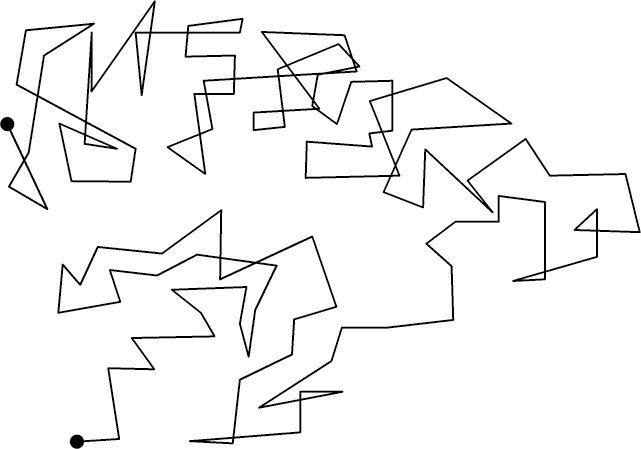
\includegraphics[scale=0.25]{brownmovement.jpg}\caption{Random Walk eines Brownschen Teilchens\footnotemark[1]}
	\end{figure}	
\end{itemize}
\footnotetext[1]{$https://www.spektrum.de/lexika/images/physik/fff1491.jpg$}
\end{frame}
\begin{frame}{Aktive Brownsche Bewegung}
\begin{itemize}
	\item beschreibt Bakterien/Zellen, die sich aus eigenem Antrieb fortbewegen
	\item Langevin-Gleichung:
	\begin{align*}
	\dot{v}=f(v)+g(v)\xi(t)
	\end{align*}
		\begin{figure}	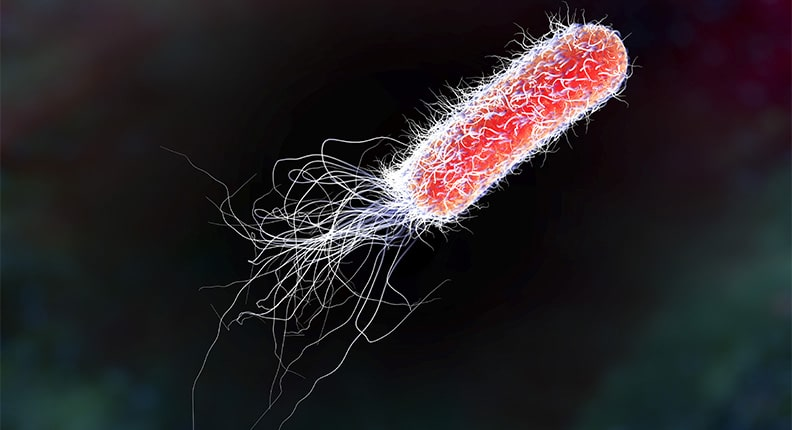
\includegraphics[scale=0.25]{ecoli.jpg}\caption{E. coli - Bakterium\footnotemark[1]}
		\end{figure}
\end{itemize}
\footnotetext[1]{$https://www.biocote.com/wp-content/uploads/2016/07/Five-Facts-about-E-coli_img.jpg$}

\end{frame}
\section{Einf"uhrung}
\begin{frame}{Gr"o"sen von Interesse}
\begin{itemize}
%\item station"are L"osung $\left(\text{mit} -U'(v)=f(v)/g^2(v)\right)$:
%\begin{equation}\nonumber
%P_0(v)=\frac{\text{e}^{-U(v)/Q}/g^2(v)}{|| \cdot ||}
%\end{equation}
\item mittlere Geschwindigkeit (Feuerrate):
\begin{align*}
\left\langle v\right\rangle =lim_{t\rightarrow\infty}\frac{\left\langle x(t)-x(0) \right\rangle}{t}\left(=\frac{\left\langle N(t) \right\rangle}{t}\right)
\end{align*}
\item Diffusionskoeffizient:
\begin{align*}
D_{eff}=lim_{t\rightarrow\infty}\frac{\left\langle x^2(t) \right\rangle-\left\langle x(t)\right\rangle ^2}{2t}\left(=\frac{\left\langle N^2(t) \right\rangle-\left\langle N(t)\right\rangle ^2}{2t}\right)
\end{align*}
\item Fano-Faktor:
\begin{align*}
F=\frac{\left\langle \Delta N^2(t) \right\rangle}{\left\langle N(t)\right\rangle}=\frac{2D_{eff}}{\langle v\rangle}
\end{align*}
\end{itemize}
\end{frame}
\section{Aktive Brownsche Teilchen}
\begin{frame}
\begin{center}
\Huge{\textcolor{darkred}{Aktive}} 

\end{center}
\begin{center}
\Huge{\textcolor{darkred}{Brownsche}}
\end{center}
\begin{center}
\Huge{\textcolor{darkred}{Teilchen}}
\end{center}
\end{frame}
\subsection{Grundlagen}
\begin{frame}{Grundlagen: Bewegungsgleichung}
\begin{itemize}
\item nichtlineare Langevin-Gleichung:
\begin{align*}\nonumber
\dot{x}&=v\\
\dot{v}&=f(v)+g(v)\xi(t)
\end{align*}
mit
\begin{equation}\nonumber
\left\langle \xi(t)\xi(t')\right\rangle =2Q\delta(t-t')
\end{equation}
\item ABP: negativer Reibungsterm $f(v)$ bei betraglich geringen Geschwindigkeiten 
\item z.B. "uber bistabiles Geschwindigkeitspotential
%\item FPE nach Ito:
%\begin{equation}\nonumber
%\frac{\partial}{\partial t}P=\frac{\partial}{\partial v}\left[-f(v)+Q\frac{\partial}{\partial v}g^2(v)\right]P
%\end{equation}
\end{itemize}
%\footnotetext[1]{L. Rondin et al., "Magnetometry with nitrogen-vacancy defects in diamond," \textit{Rep. Prog. Phys. 77}, 2014.}
\end{frame}


\subsection{Theorie}
\begin{frame}{Theorie: Modell}
\begin{itemize}
	\item Betrachtung an einfachem Modell mit $g(v)=1$ und $f(v)=v-v^3+F$\footnotemark[1]:
	\begin{align*}
	\dot{x}&=v\\
	\dot{v}&=-\frac{dU(v)}{dv}+\xi(t)
	\end{align*}
	wobei
	\begin{equation}\nonumber
		U(v)=\frac{1}{4}v^4-\frac{1}{2}v^2-Fv
	\end{equation}
	\item symmetrisch unter Inversion von $x$,$v$,$F$
	\begin{eqnarray}\nonumber
\rightarrow  \left\langle v(F)\right\rangle=-\left\langle v(-F)\right\rangle \quad\text{und}\quad D_{\text{eff}}(F)=D_{\text{eff}}(-F)
	\end{eqnarray}
\footnotetext[1]{Benjamin Lindner und Ernesto M. Nicola, "Critical Asymmetry for Giant Diffusion of Active Brownian Particles," \textit{Physical Review Letters 101}, 2008.}
\end{itemize}
\end{frame}
\begin{frame}{Theorie: Geschwindigkeitspotential}
\begin{itemize}
\item Form von $U(v)$:
	\begin{figure}	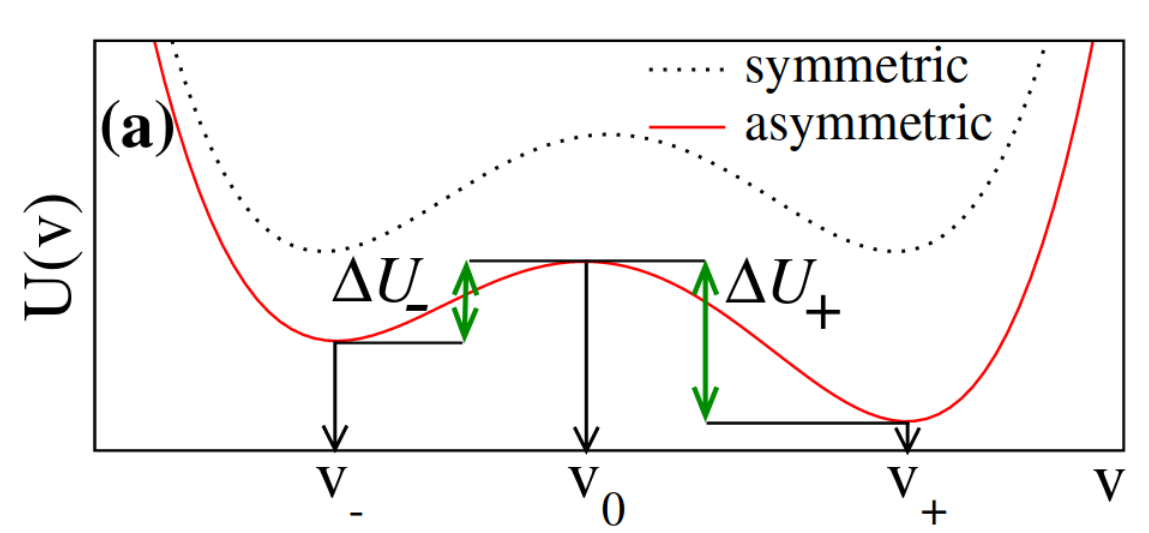
\includegraphics[height=3.5cm]{velpot.png}\caption{Geschwindigkeitspotential im vereinfachten Modell}
	\end{figure}
\item 2 Minima bei $v_-$ und $v_+$ mit zugeh"origen Barrieren $\Delta U_{\pm}=U(v_0)-U(v_{\pm})$	
\end{itemize}
\end{frame}
\begin{frame}{heorie: Geschwindigkeitspotential}
\begin{itemize}
\item bistabiles Geschwindigkeitspotential ruft bidirektionale Bewegung hervor
\end{itemize}
\begin{figure}	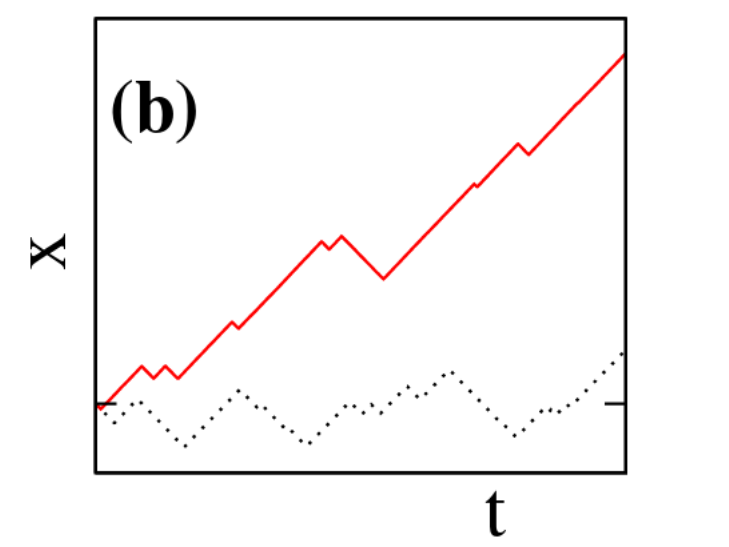
\includegraphics[height=3.5cm]{xt.png}\caption{x-t-Diagramm bei symmetrischem und asymmetrischem Geschwindigkeitspotential}
\end{figure}
\begin{itemize}
\item Asymmetrie f"uhrt zu nichtverschwindendem $\left<v\right>$	
\end{itemize}
\end{frame}
\subsection{Simulation}
\begin{frame}{Simulation}
	\begin{figure}	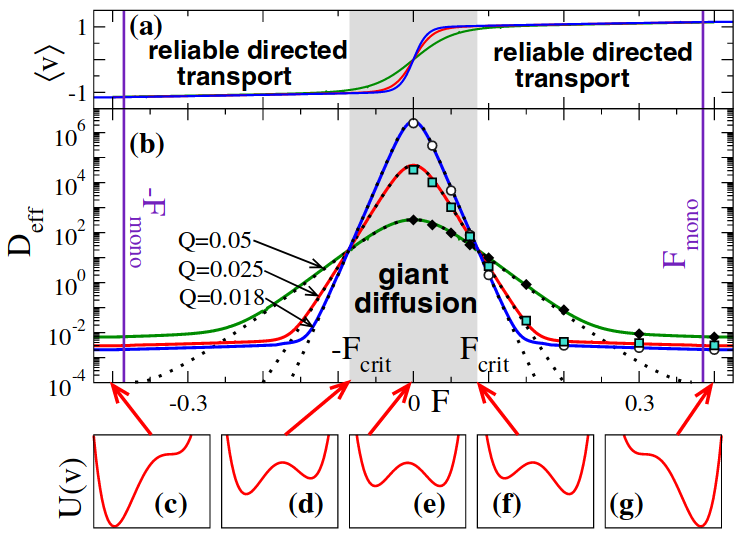
\includegraphics[height=6cm]{mess08.png}\caption{Bestimmung von Geschwindigkeit und Diffusionskoeffizient}
	\end{figure}
\end{frame}
\subsection{Zwei-Zustands-System}
\begin{frame}{Zwei-Zustands-System}
\begin{itemize}
	\item geringes Rauschen: Verhalten des Systems durch "Ubergange zwischen Zust"anden bestimmt
	\item f"ur "Ubergangsraten wird Arrhenius-Gleichung angenommen:
\end{itemize}
\begin{align*}
r_{\pm}=r_{0,\pm}\text{e}^{-\frac{\Delta U_{\pm}}{Q}}
\end{align*}
\begin{itemize}
	\item $r_-$: r"uckw"arts zu vorw"arts, $r_+$ umgekehrt, $Q$: Rauschintensit"at
\item $D_{\text{eff}}$ aus Raten und $\Delta v=v_+-v_-$:
\end{itemize}
\begin{align*}
D_{\text{eff}}=\frac{(\Delta v)^2 r_+r_-}{(r_++r_-)^3}
\end{align*}
\end{frame}
\begin{frame}{Zwei-Zustands-System}
\begin{itemize}
	\item gesucht: $F_{crit}$
	\item nahe Schnittpunkt: $D_{\text{eff}}(Q,F)$=$D_{\text{eff}}(F)$
	\item Einsetzen:
\begin{align*}
D_{\text{eff}}&=\frac{(\Delta v)^2r_{0,+}r_{0,-}\text{e}^{-\frac{\Delta U_++\Delta U_-}{Q}}}{\left(r_{0,+}\text{e}^{\frac{-\Delta U_+}{Q}}+r_{0,-}\text{e}^{\frac{-\Delta U_-}{Q}}\right)^3}\\&=\frac{(\Delta v)^2r_{0,+}r_{0,-}}{\left(r_{0,+}\text{e}^{-\frac{3\Delta U_+-\Delta U_+-\Delta U_-}{3Q}}+r_{0,-}\text{e}^{-\frac{3\Delta U_--\Delta U_+ -\Delta U_-}{3Q}}\right)^3}\\&=\frac{(\Delta v)^2r_{0,+}r_{0,-}}{\left(r_{0,+}\text{e}^{-\frac{2\Delta U_+-\Delta U_-}{3Q}}+r_{0,-}\text{e}^{-\frac{2\Delta U_--\Delta U_+}{3Q}}\right)^3}
\end{align*}
\end{itemize}
\end{frame}
\begin{frame}{Zwei-Zustands-System}
\begin{itemize}
	\item Grenzfall $Q\rightarrow 0,\Delta U_+>\Delta U_-$:
\begin{align*}
D_{\text{eff}}=\frac{(\Delta v)^2r_{0,+}}{r_{0,-}^2}\text{e}^{-\frac{\Delta U_+-2\Delta U_-}{Q}}
\end{align*}
\item bei $\left|\frac{d}{dF}\left(\frac{(\Delta v)^2r_{0,+}}{r_{0,-}^2}\right)/\frac{d}{dF}D_{\text{eff}} \right| \ll 1$:
\begin{align*}
\Delta U_+=2\Delta U_-
\end{align*}
\item symmetrisches Problem $\rightarrow$ 2. Schnittpunkt bei
\begin{align*}
\Delta U_-=2\Delta U_+
\end{align*}
\item $\Delta U_\pm =2\Delta U_\mp$
\end{itemize}
\end{frame}
%\begin{frame}{Zwei-Zustands-System}
%\begin{itemize}
%	\item Kriterium f"uhrt auf interessante Eigenschaft von $P_0(v)$
%	\item betrachte Verh"altnis aus $P_0(v)$ an Extremstellen:
%	\begin{align*}
%	R_p(F,Q)=\frac{P_0(v_0)P_0(v_+)}{P_0^2(v_-)}
%	\end{align*}
%	\item setze Schnittpunktbedingung ein:
%	\begin{align*}
%	R_p(F,Q)&=\frac{\text{e}^{-U(v_0)/Q}}{g^2(v_0)}\frac{\text{e}^{-U(v_+)/Q}}{g^2(v_+)}\frac{g^4(v_-)}{\text{e}^{-2U(v_-)/Q}}\\
%	&=\text{e}^{\left[2U(v_-)-2U(v_0)-(U(v_+)-U(v_0))\right]/Q}\frac{g^4(v_-)}{g^2(v_0)g^2(v_+)}\\&=\frac{g^4(v_-)}{g^2(v_0)g^2(v_+)}
%	\end{align*} 
%\end{itemize}
%\end{frame}
%\section{Gekoppelte Molekulare Motoren}
%\begin{frame}
%\begin{center}
%	\Huge{\textcolor{darkred}{Gekoppelte}} 
%	
%\end{center}
%\begin{center}
%	\Huge{\textcolor{darkred}{Molekulare}}
%\end{center}
%\begin{center}
%	\Huge{\textcolor{darkred}{Motoren}}
%\end{center}
%\end{frame}
%\subsection{Theorie}
%\begin{frame}{Theorie: Potential}
%\begin{figure}	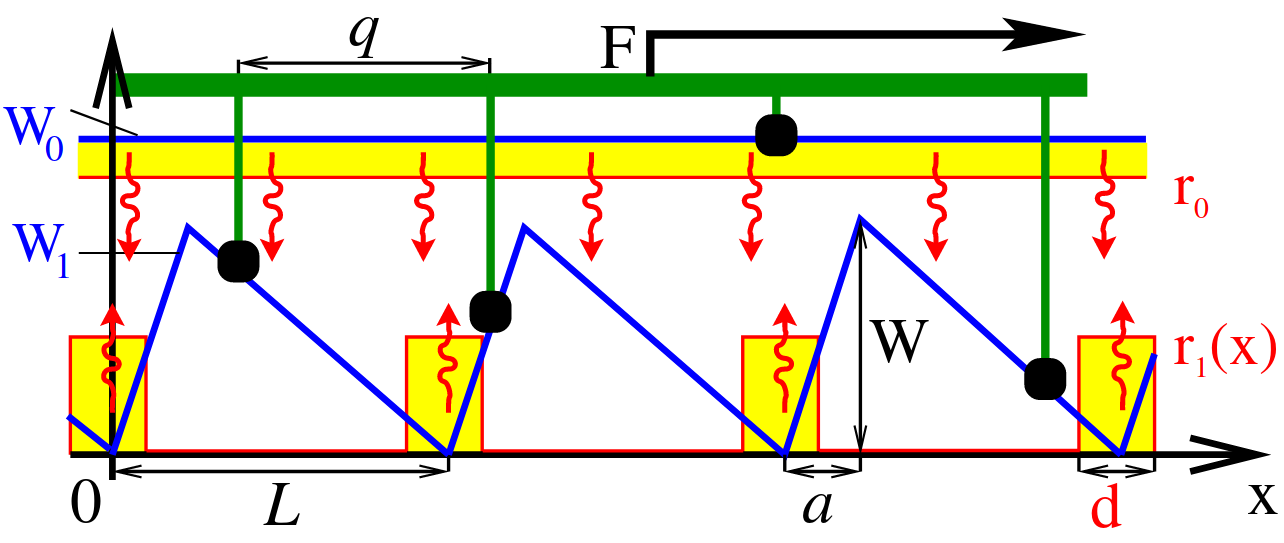
\includegraphics[height=5cm]{coupledmolmot.png}\caption{Gekoppelte molekulare Motoren. Gr"un: Ger"ust mit "aquidistant befestigten Motoren, Blau: zustands-u. ortsabh"angige Potentiale $W_{\sigma_i}$, Gelb: Raten $r_0$(0 $\rightarrow$ 1) und $r_1$(1 $\rightarrow$ 0)}
%\end{figure}
%\end{frame}
%\begin{frame}{Theorie: Bewegungsgleichung}
%\begin{itemize}
%	\item Kraft durch die Motoren:
%	\begin{align*}
%F_{mot}=-\sum_{i=1}^{N}\partial_xW_{\sigma_i}(x_i)
%	\end{align*}
%	\item Bewegungsgleichung des R"uckgrats 
%	\begin{align*}
%\dot{x}=\frac{1}{\lambda}\left[f_{mot}+f_{ext}+\eta(t)\right]
%	\end{align*}
%	mit 
%\begin{align*}
%	f_{mot}&=F_{mot}/N\\
%	f_{ext}&=F_{ext}/N\\ \left<\eta(t)\eta(t')\right>&=(2k_BT\lambda/N)\delta(t-t')
%\end{align*}
%\end{itemize}
%\end{frame}
%\subsection{Simulation}
%\begin{frame}{Simulation mit symmetrischem Potential}
%\begin{tikzpicture}
%\node (img1)[xshift=0cm][yshift=0cm] {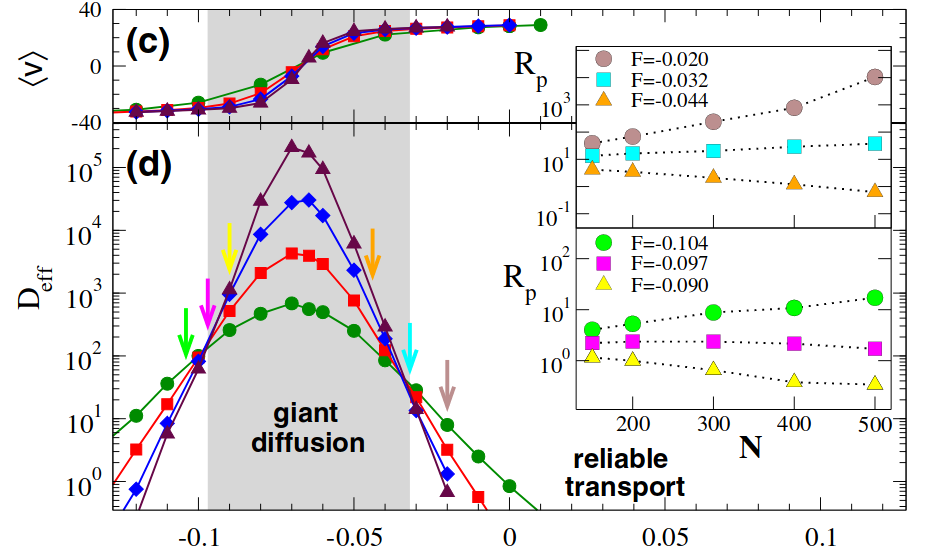
\includegraphics[scale=0.335]{molmotsim2.png}};
%\node (img2) at (img1.north west)[yshift=-3.2cm][xshift=5.62cm] {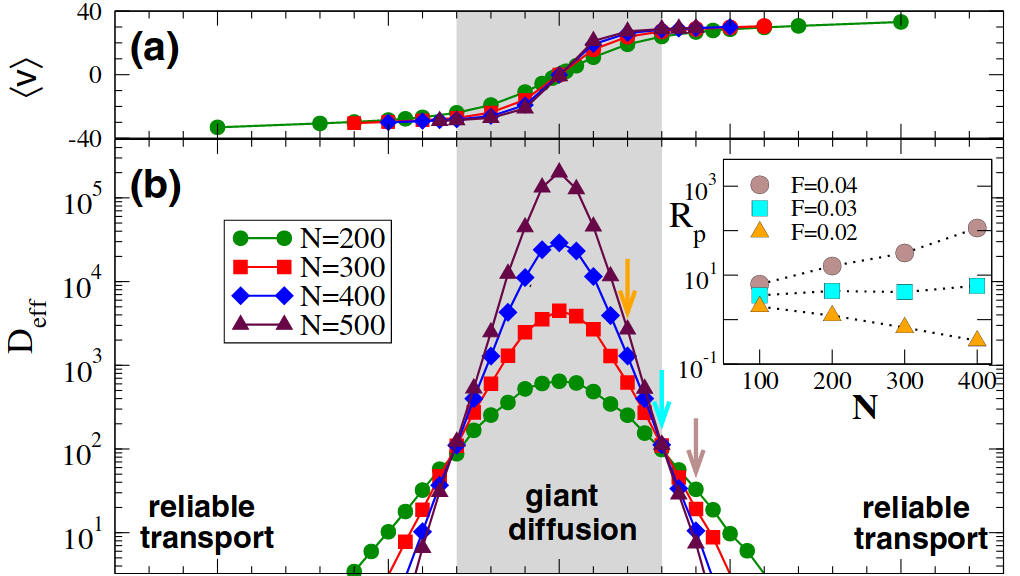
\includegraphics[scale=0.3]{molmotsim1.png}};
%\end{tikzpicture}
%\end{frame}
%\subsection{Simulation}
%\begin{frame}{Simulation mit asymmetrischem Potential}
%\begin{figure}	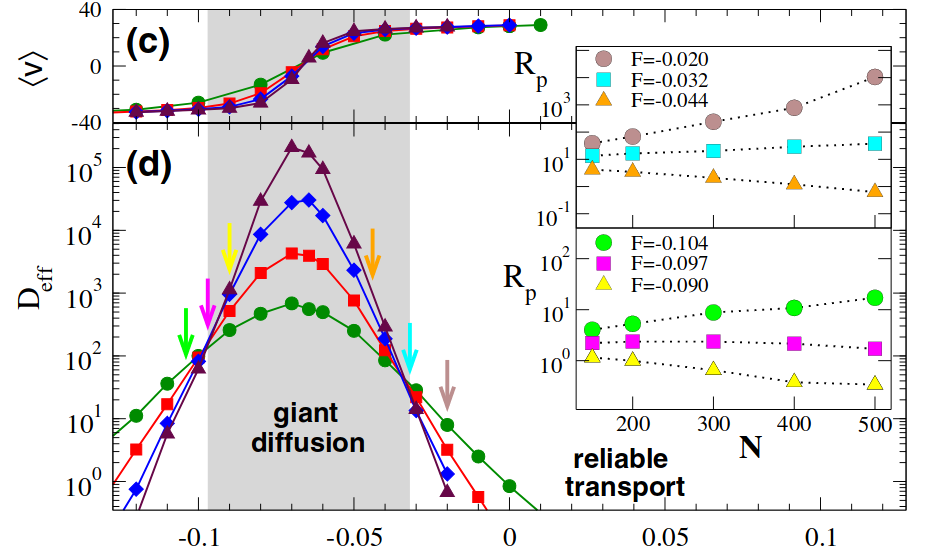
\includegraphics[scale=0.33]{molmotsim2.png}\
%\end{figure}
%\end{frame}
\section{Brownsche Teilchen im gekippten Kosinuspotential}
\begin{frame}
\begin{center}
	\Huge{\textcolor{darkred}{Brownsche}}
\end{center}
\begin{center}
	\Huge{\textcolor{darkred}{Teilchen}}
\end{center}
\begin{center}
	\Huge{\textcolor{darkred}{im gekippten}}
\end{center}
\begin{center}
	\Huge{\textcolor{darkred}{periodischen}}
\end{center}
\begin{center}
	\Huge{\textcolor{darkred}{Potential}}
\end{center}
\end{frame}
\subsection{Theorie}
\begin{frame}{Theorie: Bewegungsgleichungen}
\begin{itemize}
	\item Langevin-Gleichung:
	\begin{align*}
\dot{x}&=v\\
\dot{v}&=-\gamma v -U'(x)+\sqrt{2\gamma kT}\xi(t)
	\end{align*}
	mit\footnotemark[1]
	\begin{align*}
U(x)=-Fx-d\cos(x)
	\end{align*}
	\item $\gamma$: Reibungskoeffizient, $\left<\xi(t)\xi(t')\right>=\delta(t-t')$, $d=1$
\end{itemize}
\footnotetext[1]{Benjamin Lindner und Igor M. Sokolov, "Giant diffusion of underdamped particles in a biased periodic potential," \textit{Physical Review E 93}, 2016.}
\end{frame}
\begin{frame}{Theorie - Potential}
\begin{columns}[t]
	\column{.5\textwidth}
	\centering
	\vspace{-2.5cm}
\begin{figure}	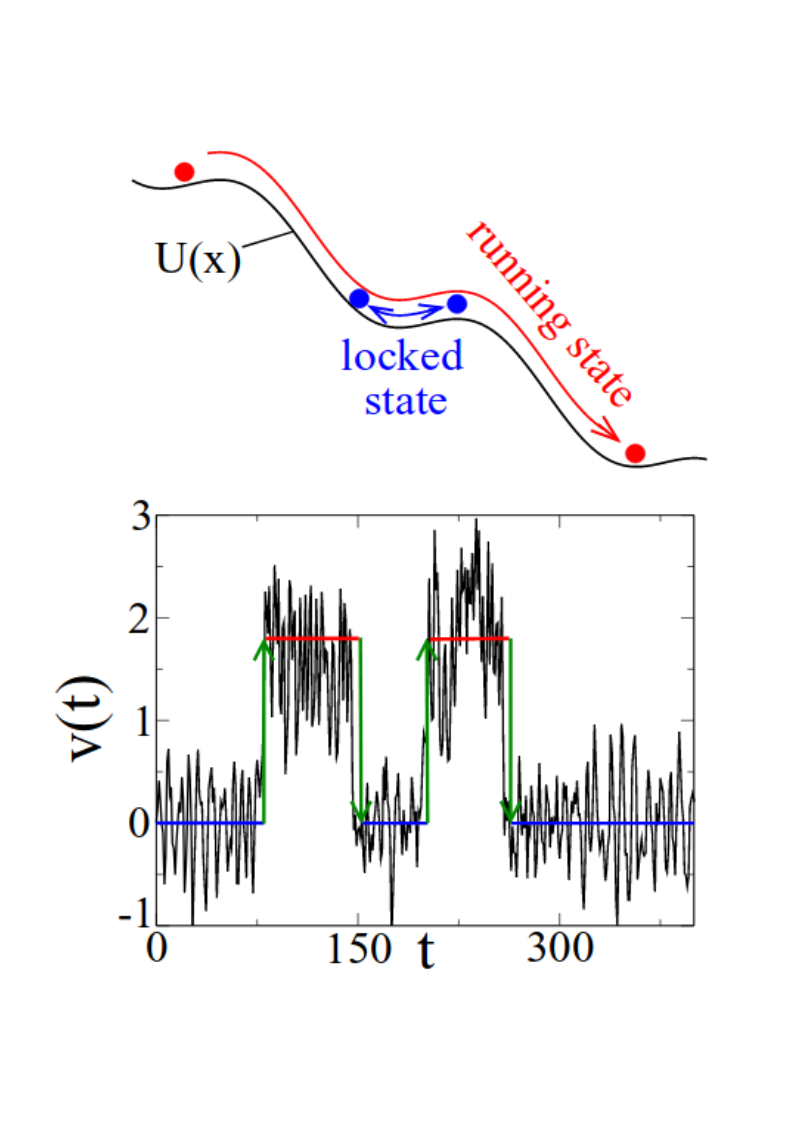
\includegraphics[scale=0.33]{nbpveldyncor.png}\
\end{figure}
	\column{.5\textwidth}
	\begin{itemize}
		\item Bewegung von Kugeln in einem gekippten Kosinuspotential 
	\end{itemize}
\bigskip\bigskip\bigskip\bigskip
\begin{itemize}
	\item Bistabilit"at der Geschwindigkeit
\end{itemize}
\end{columns}
\end{frame}
\subsection{Simulation}
\begin{frame}{Simulation: Diffusionskoeffizient}
\begin{figure}	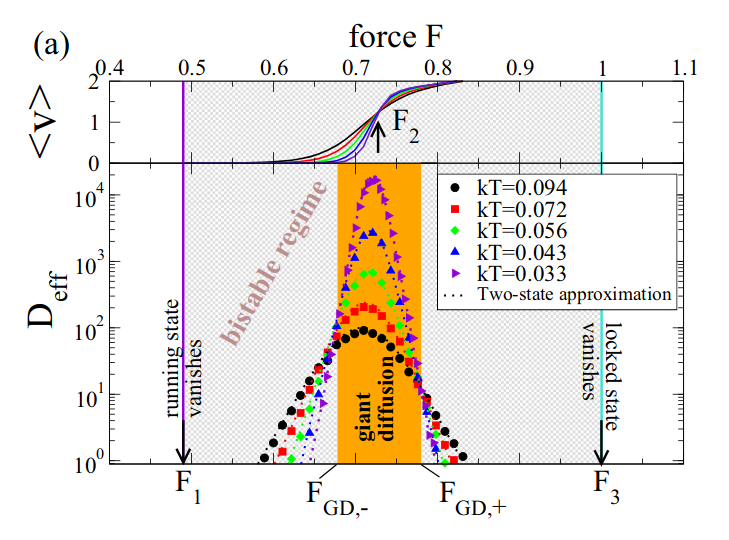
\includegraphics[scale=0.4]{nbpsim1.png}\
\end{figure}
\end{frame}
\begin{frame}{Simulation - kritischer Bereich}
\begin{figure}	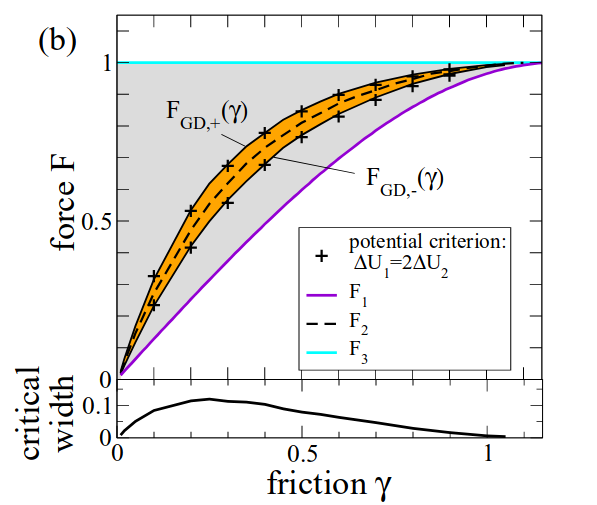
\includegraphics[scale=0.4]{nbpsim2.png}\
\end{figure}
\end{frame}
\subsection{Auswertung}
\begin{frame}{Berechnung effektiver Potentialbarrieren}
\begin{itemize}
	\item Annahme: "Ubergangsraten zeigen Kramers-"ahnliches Verhalten:
	\begin{align*}
r\propto T^\alpha \text{e}^{-\frac{\Delta U}{kT}}
	\end{align*}

	\begin{figure}	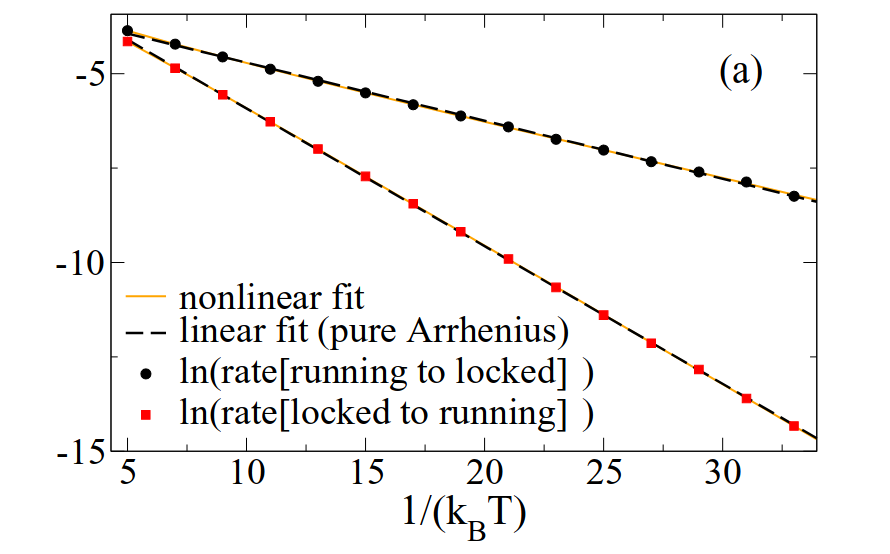
\includegraphics[scale=0.25]{kramerfit.png}\
	\end{figure}	
\item Fits f"ur $\alpha=0$ und $\alpha \neq 0$ liefern "ahnliche Barrieren
	\end{itemize}
\end{frame}
\begin{frame}{Berechnung effektiver Potentialbarrieren}
\begin{itemize}
	\item Plotten von $\Delta U$ und $2\Delta U$ f"ur verschiedene Kr"afte 
	\begin{figure}	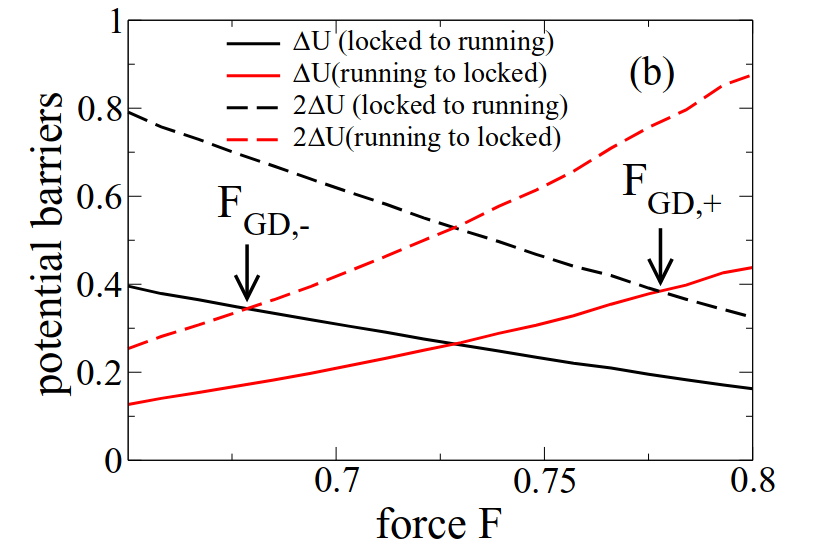
\includegraphics[scale=0.25]{barrierplot.png}\
	\end{figure}	
	\item Schnittpunkte etwa bei $F=0.68$ und $F=0.78$ 
\end{itemize}
\end{frame}
\begin{frame}{Berechnung effektiver Potentialbarrieren}
\begin{itemize}
	\item Vergleich mit Simulation
	\begin{figure}	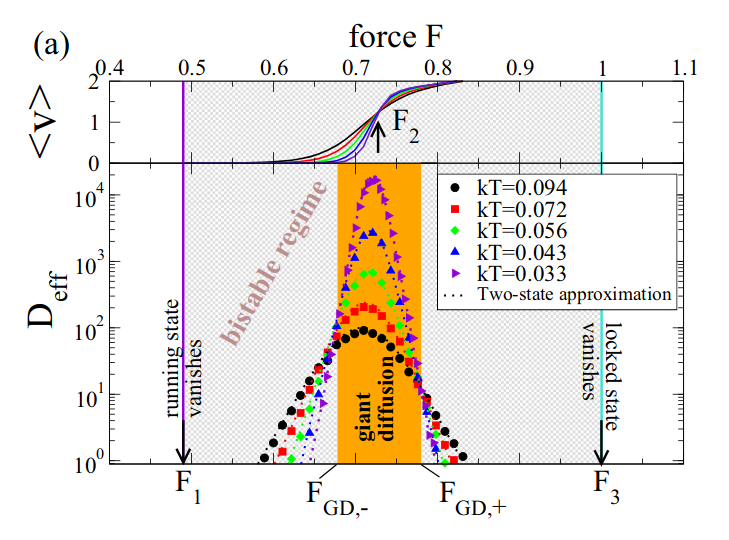
\includegraphics[scale=0.37]{nbpsim1.png}\
	\end{figure}	
\end{itemize}
\end{frame}
\subsection{Reproduktion}
\begin{frame}{Reproduktion: Geschwindigkeit}
\begin{figure}	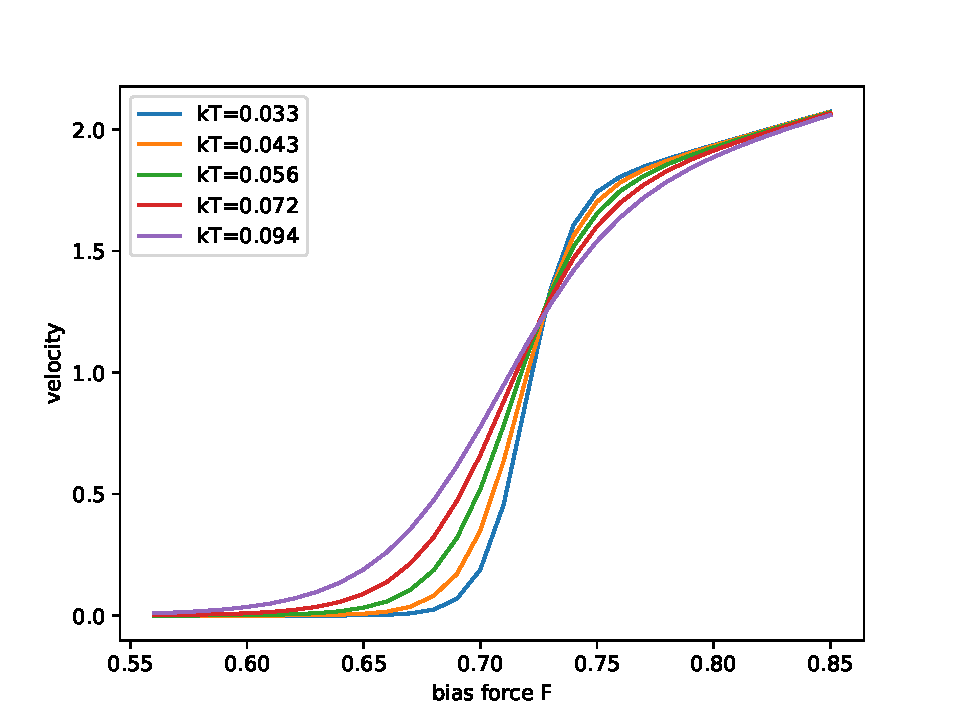
\includegraphics[scale=0.6]{gmechexaktnew.pdf}\
\end{figure}
\end{frame}
\begin{frame}{Reproduktion: Diffusionskoeffizient}
\begin{figure}	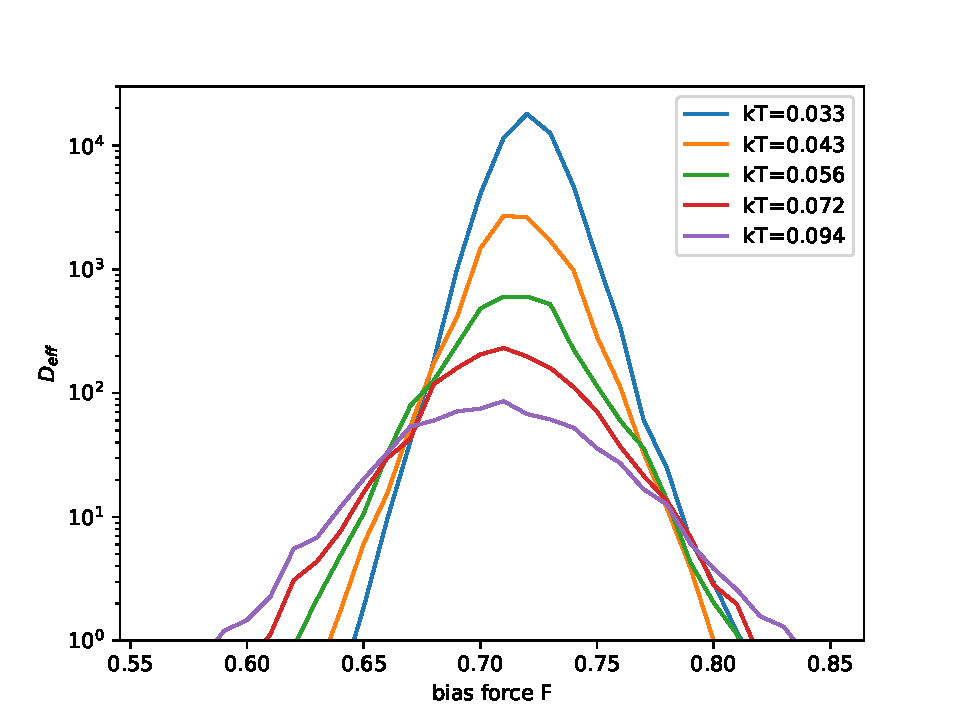
\includegraphics[scale=0.6]{dmechexaktnew.pdf}\
\end{figure}
\end{frame}
\begin{frame}{Reproduktion: Fano - Faktor}
\begin{figure}	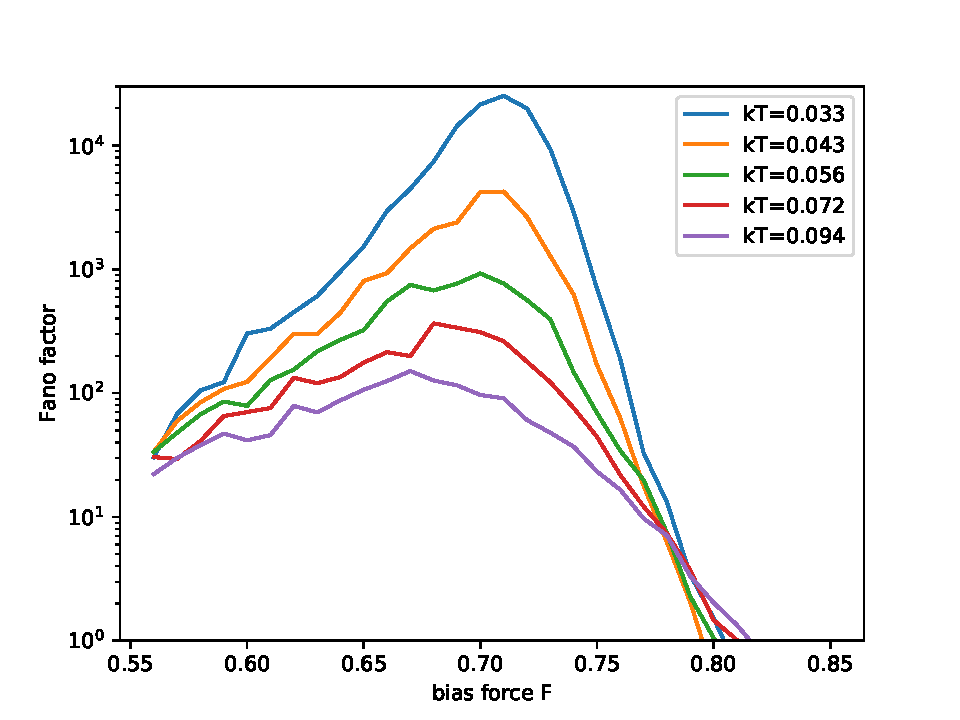
\includegraphics[scale=0.6]{fmechexaktnew.pdf}\
\end{figure}
\end{frame}
\subsection{Zwei-Zustands-System}
\begin{frame}{Zwei-Zustands-System}
\begin{itemize}
	\item gesucht: m"ogliche Schnittpunkte im Fano-Faktor
	\begin{align*}
	F=\frac{2D_{\text{eff}}}{\left<v\right>}
	\end{align*}
	\item Mittelwert der Geschwindigkeit:
	\begin{align*}
	\left<v\right>=v_+\frac{r_-}{r_++r_-}
	\end{align*}
	\item Einsetzen der "Ubergangsraten:
	\begin{align*}
	F&=\frac{2v_+r_+}{(r_++r_-)^2}=\frac{2v_+r_{0,+}\text{e}^{-\frac{\Delta U_+}{Q}}}{\left(r_{0,+}\text{e}^{-\frac{\Delta U_+}{Q}}+r_{0,-}\text{e}^{-\frac{\Delta U_-}{Q}}\right)^2}\\
	&=\frac{2v_+r_{0,+}}{\left(r_{0,+}\text{e}^{-\frac{2\Delta U_+-\Delta U_+}{2Q}}+r_{0,-}\text{e}^{-\frac{2\Delta U_--\Delta U_+}{2Q}}\right)^2}
	\end{align*}
\end{itemize}
\end{frame}
\begin{frame}{Zwei-Zustands-System}
\begin{itemize}
	\item Grenzfall $Q\ll1$ $\rightarrow$ zwei L"osungen
	\item $\Delta U_+ > \Delta U_-$:
	\begin{align*}
	F=\frac{2v_+r_{0,+}}{r_{0,-}^2}\text{e}^{-\frac{\Delta U_+-2\Delta U_-}{Q}} \rightarrow \Delta U_+=2\Delta U_-
	\end{align*}
	\item $\Delta U_+ < \Delta U_-$:
	\begin{align*}
	F=\frac{2v_+}{r_{0,+}}\text{e}^{-\frac{\Delta U_+-2\Delta U_+}{Q}} \rightarrow \Delta U_+=0
	\end{align*}
	\item eine Barriere muss verschwinden $\rightarrow$ Rand des G"ultigkeitsbereichs der Zwei-Zustands-Theorie erreicht
	\item rechter Schnittpunkt bleibt erhalten, linker verschiebt sich weiter nach links
\end{itemize}
\end{frame}
\section{Nervenmodell}
\begin{frame}
\begin{center}
	\Huge{\textcolor{darkred}{Nervenmodell}}
\end{center}
\end{frame}
\begin{frame}{"Ubergang Brownsche Teilchen $\rightarrow$ Nervenmodell}
\begin{figure}	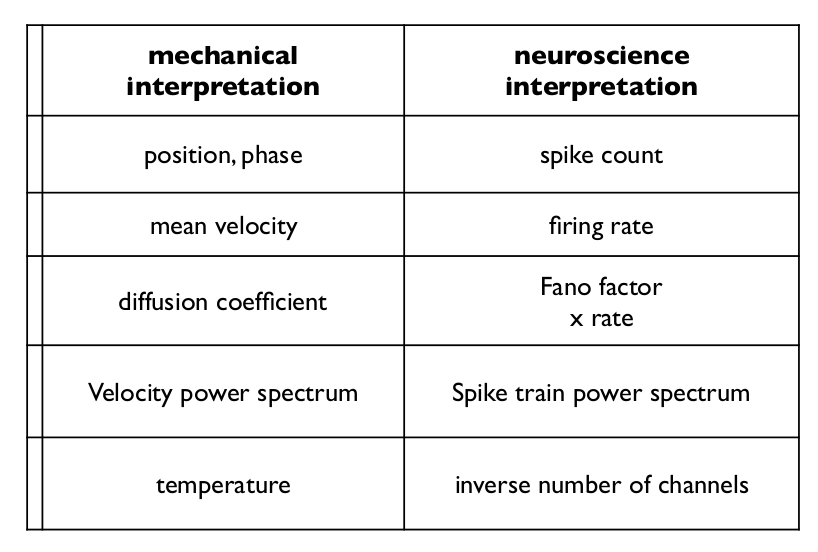
\includegraphics[scale=0.4]{ubergang.png}
\end{figure}
\end{frame}
\subsection{Theorie}
\begin{frame}{Theorie: Modell}
\begin{adjustwidth}{-1em}{-1em}
\begin{itemize}
	\item $I_{Na,p}+I_K$-Modell:
\begin{align*}
C\dot{V} &= I - g_L(V-E_L) - g_{Na}m_{\infty}(V)(V-E_{Na}) - g_Kn(V-E_K)+\sqrt{2D}\xi(t)\\
\dot{n} &= (n_{\infty}(V)-n)/\tau(V)
\end{align*}
\item Steady-State-Aktivierungsfunktion:
\begin{align*}
f_{\infty}(V) = \frac{1}{1+\exp\{(V_{1/2}-V)/k\}}
\end{align*}
\item hierbei ist k die Steigung, sowie:
\begin{align*}
f_{\infty}(V_{1/2})=1/2
\end{align*}
\end{itemize}
\end{adjustwidth}
\end{frame}
\subsection{Deterministisches Verhalten}

\begin{frame}{Deterministisches Verhalten: Bursten}
%\begin{itemize}
%	\item burstende Anfangsbedingungen
\begin{figure}	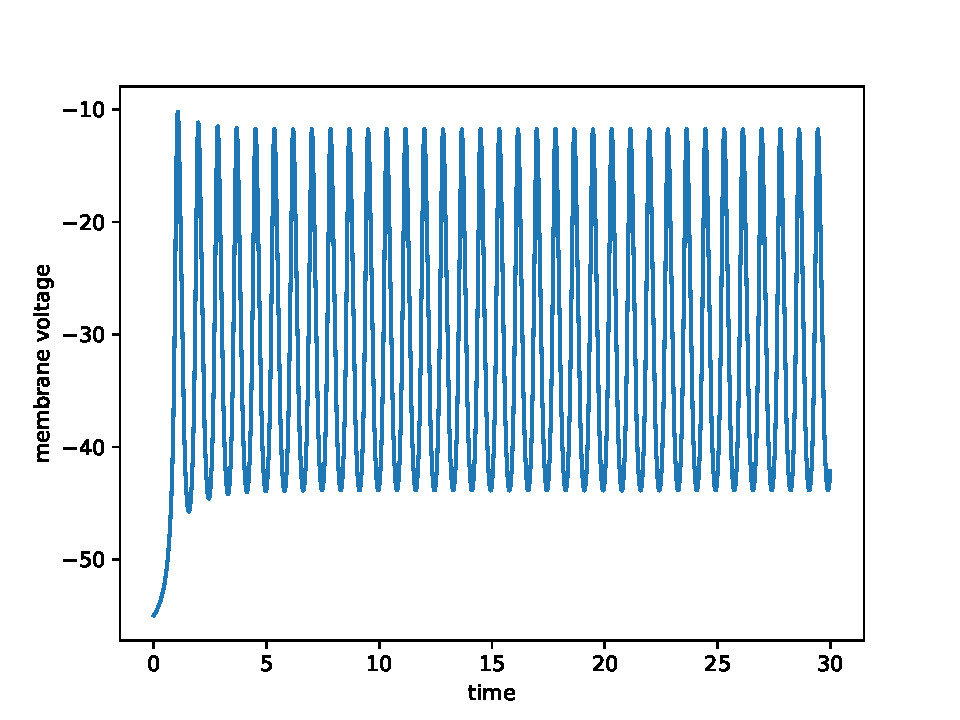
\includegraphics[scale=0.6]{inapi0d0.pdf}
\end{figure}
%\end{itemize}
\end{frame}
\begin{frame}{Deterministisches Verhalten: Bursten}
%\begin{itemize}
%	\item burstende Anfangsbedingungen
	\begin{figure}	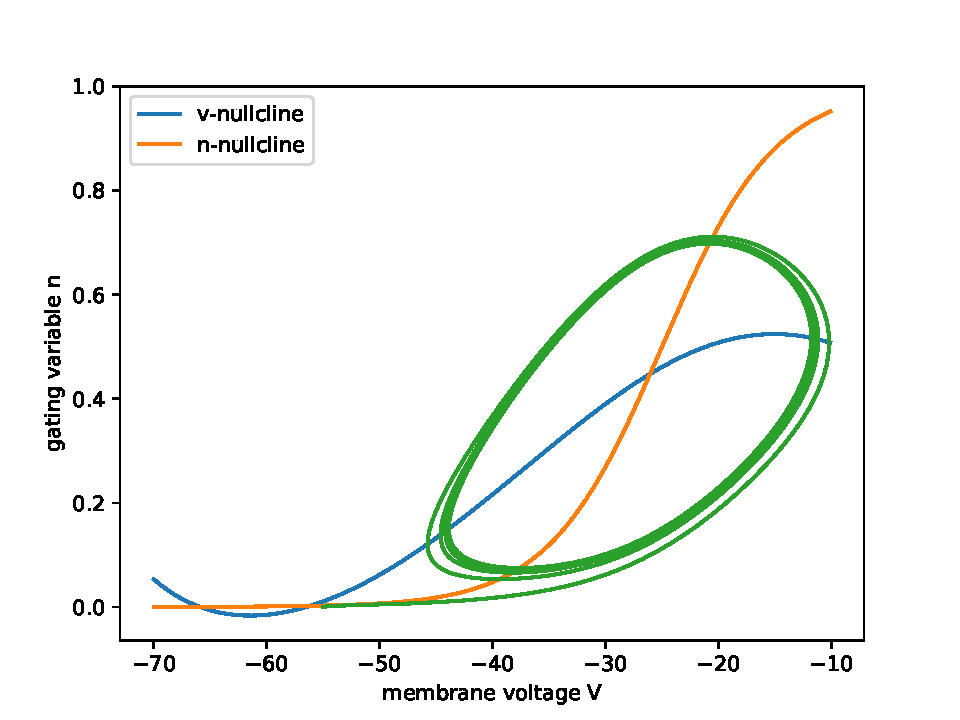
\includegraphics[scale=0.6]{inapburstwn.pdf}
	\end{figure}
%\end{itemize}
\end{frame}
\begin{frame}{Deterministisches Verhalten: Ruhen}
%\begin{itemize}
%	\item nicht burstende Anfangsbedingungen
	\begin{figure}	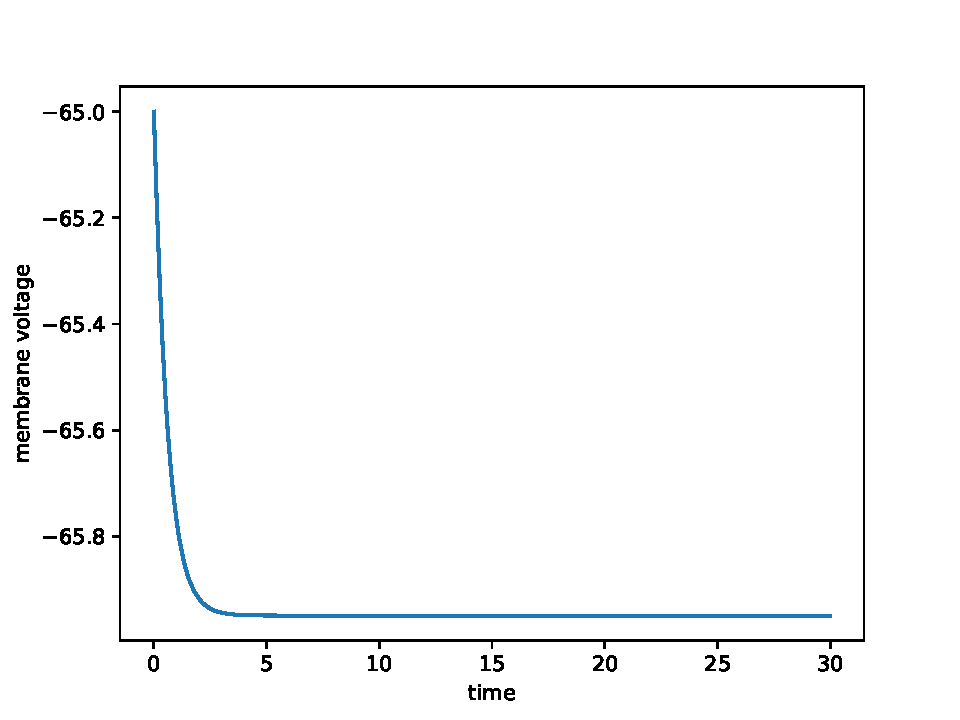
\includegraphics[scale=0.6]{inapnbi0d0.pdf}
	\end{figure}
%\end{itemize}
\end{frame}
\begin{frame}{Deterministisches Verhalten: Ruhen}
%\begin{itemize}
%	\item nicht burstende Anfangsbedingungen
\begin{tikzpicture}
\node (img1)[xshift=0cm][yshift=0cm] {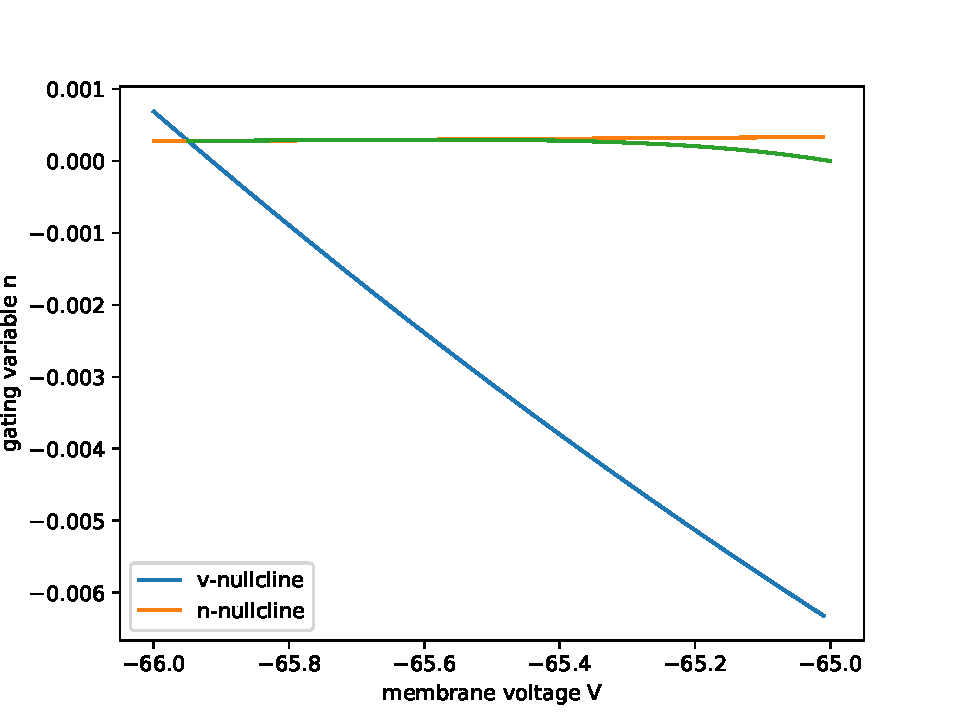
\includegraphics[scale=0.635]{inapnoburstwn.pdf}};
\node (img2) at (img1.north west)[yshift=-3.8cm][xshift=9.62cm] {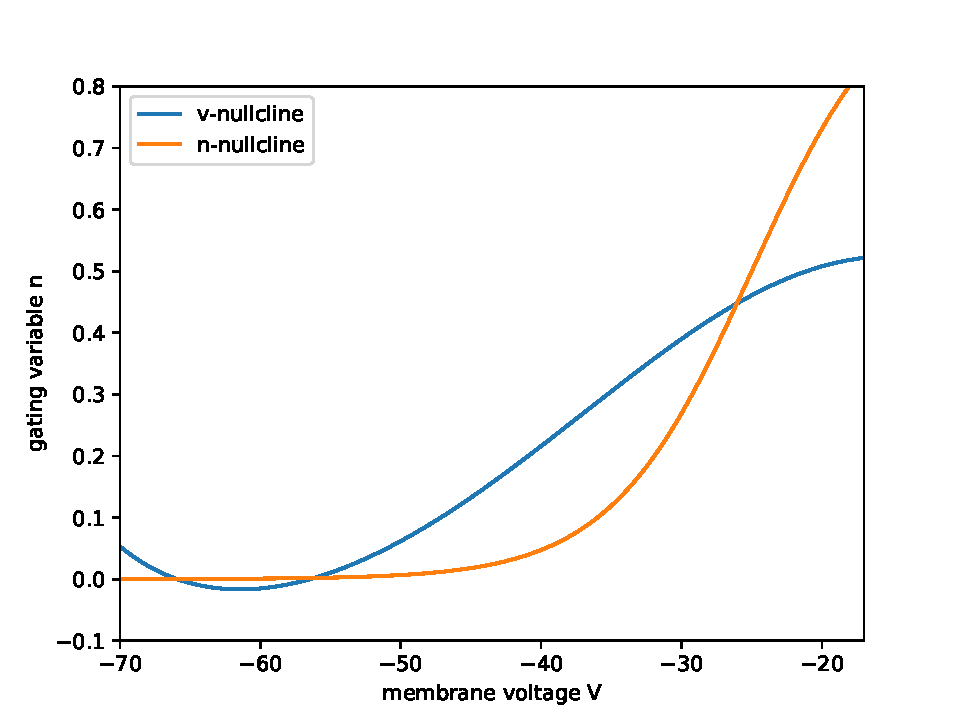
\includegraphics[scale=0.28]{inapikncpure.pdf}};
\end{tikzpicture}
%\end{itemize}
\end{frame}
\subsection{Verhalten unter Rauschen}
\begin{frame}{Verhalten unter Rauschen}
\begin{columns}[t]
	\column{.5\textwidth}
	\centering
	\vspace{-1cm}
	\begin{figure}
		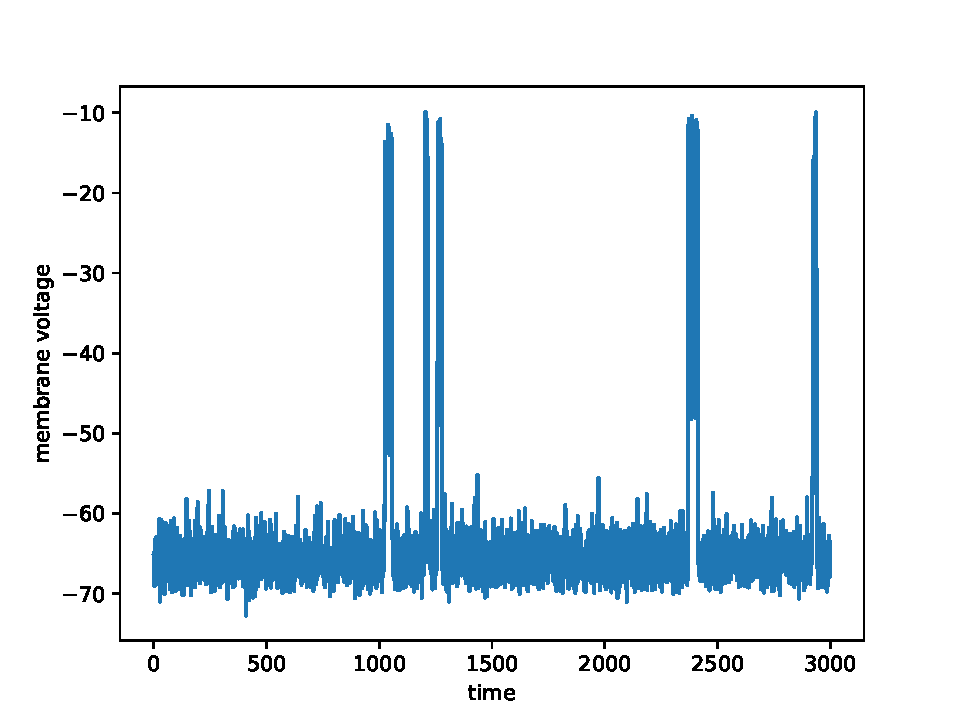
\includegraphics[scale=0.3]{inapni0d5.pdf}
	\end{figure}
\vspace{-1cm}
	\begin{figure}
	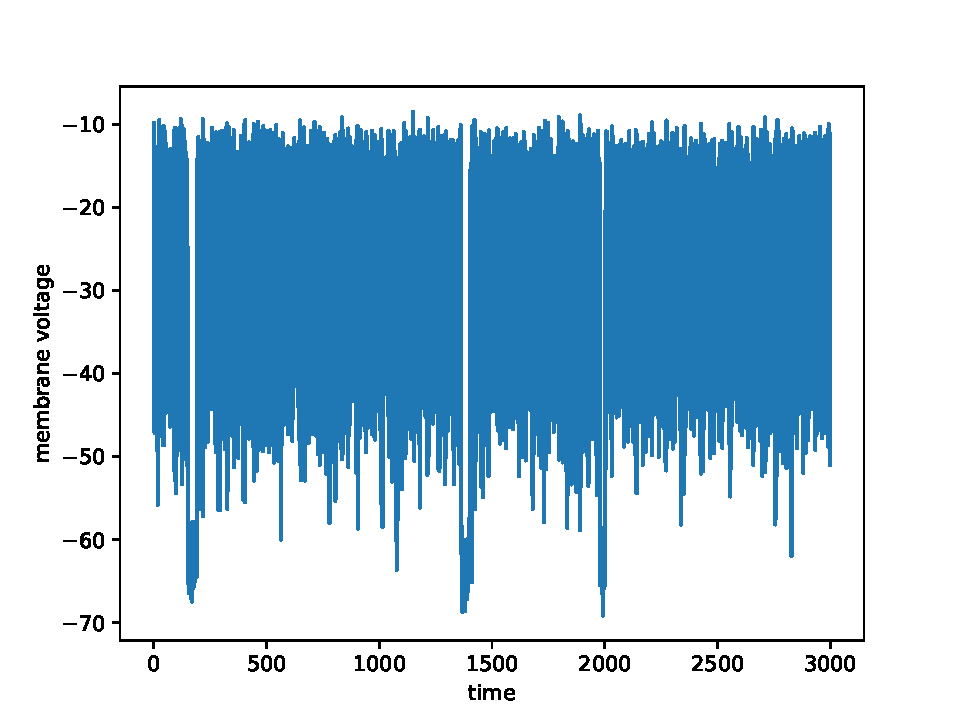
\includegraphics[scale=0.3]{inapi3d5.pdf}
\end{figure}
	\column{.5\textwidth}
	\centering
	\vspace{-0.5cm}
	\begin{figure}
		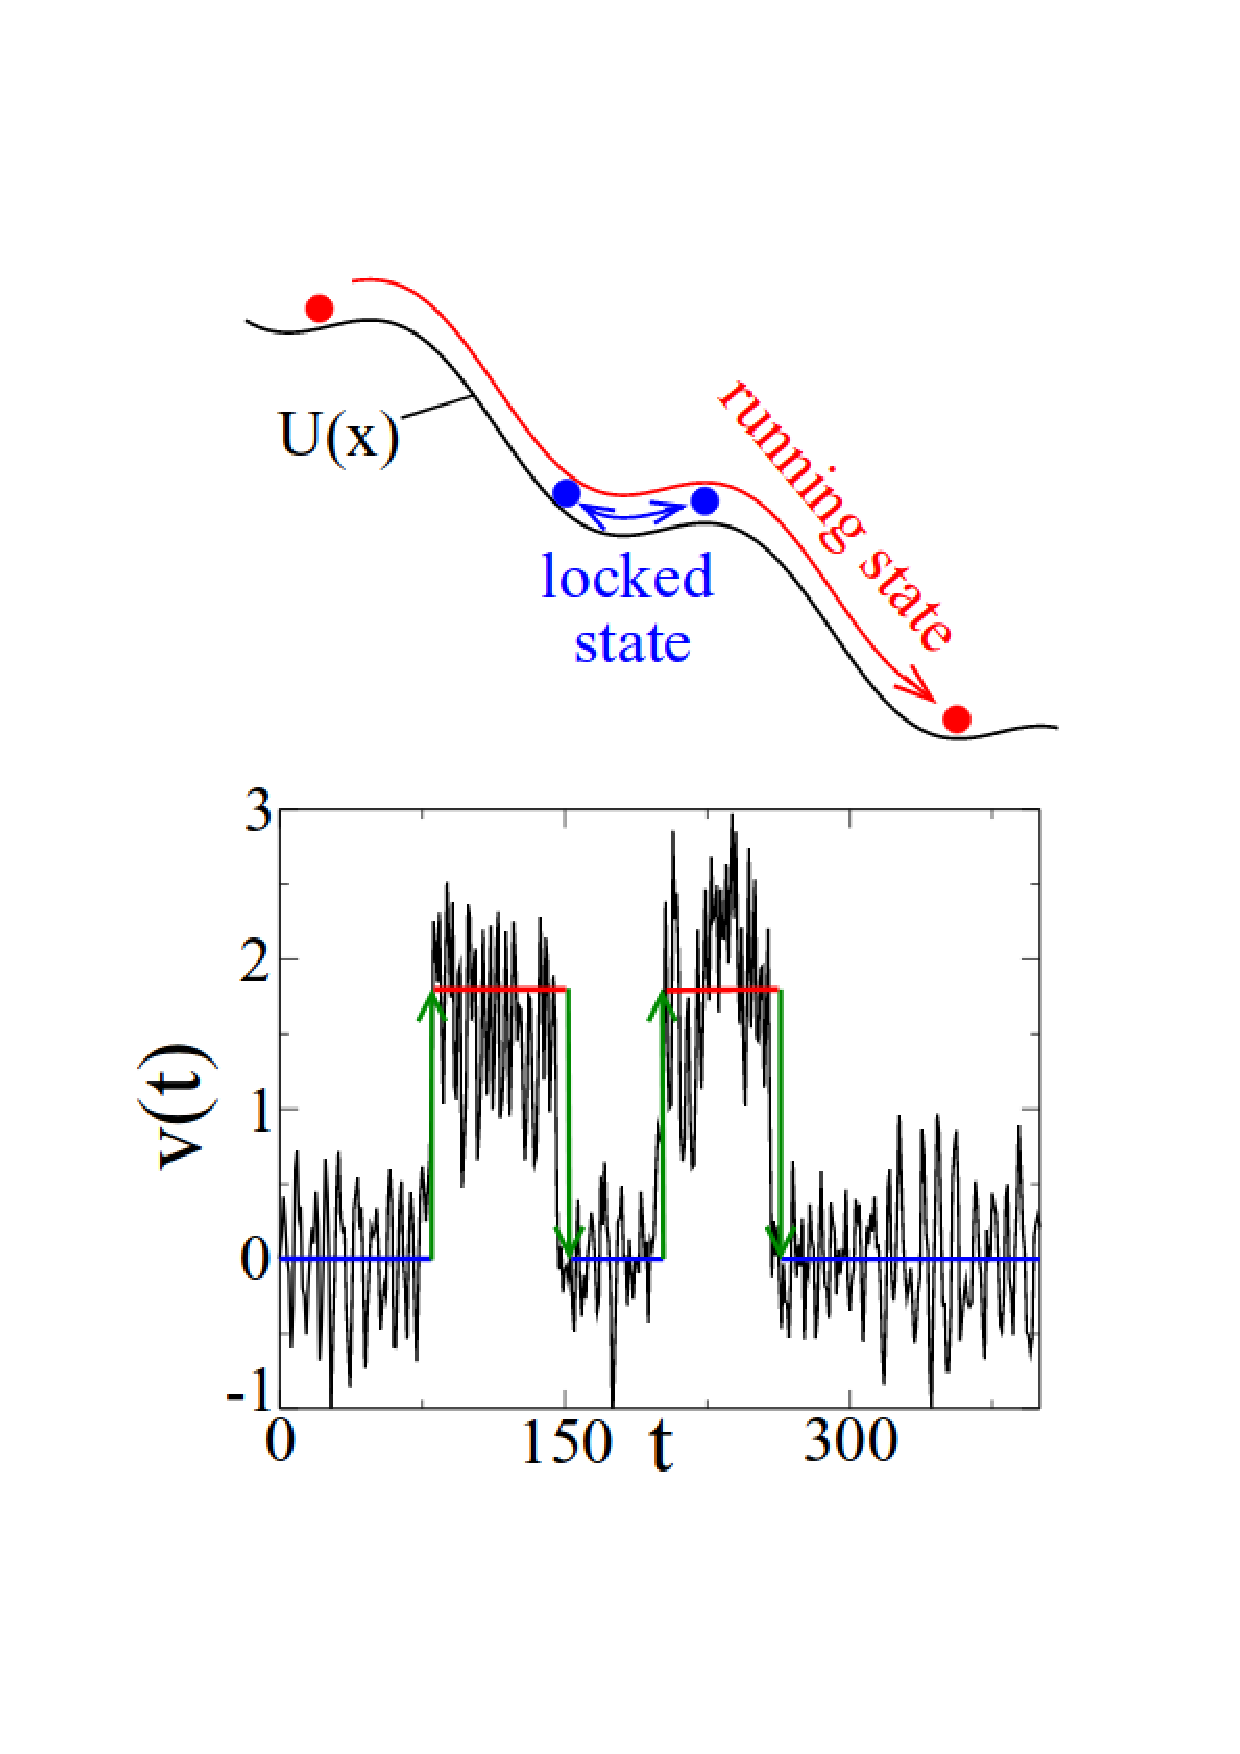
\includegraphics[scale=0.25]{nbpveldyncor.pdf}
	\end{figure}\vspace{-8.7cm}
	\begin{figure}
	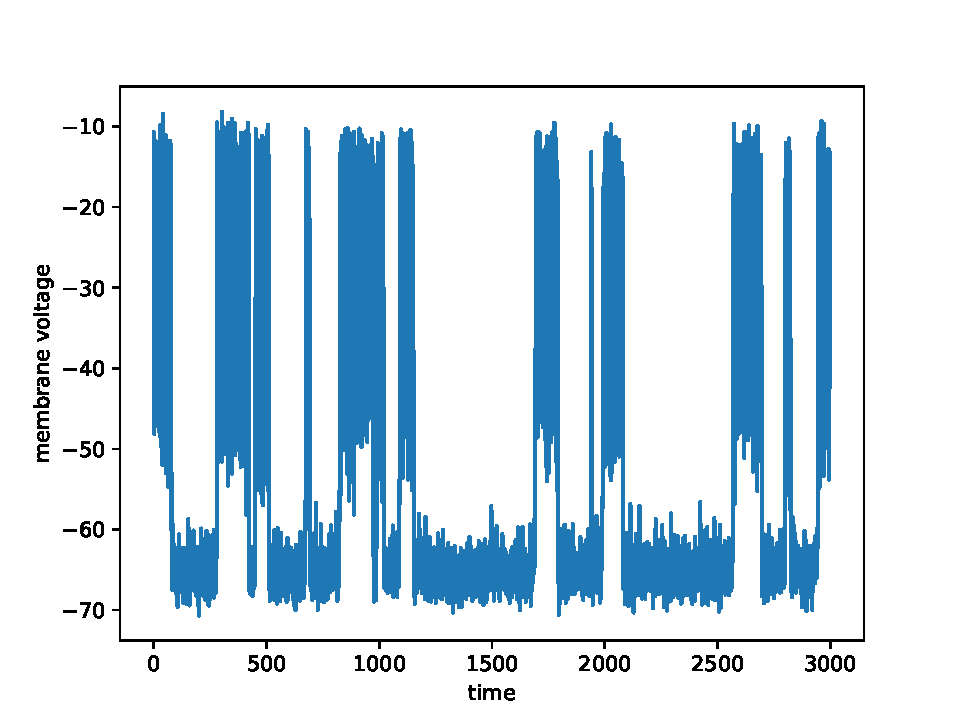
\includegraphics[scale=0.3]{inapi1d5.pdf}
\end{figure}
%\begin{itemize}
%	\item links oben: rauschinduzierte "Uberg"ange bei $I=0$
%	\item rechts oben: I=1
%	\item links unten: I=3
%\end{itemize}
\end{columns}
\end{frame}
\subsection{Simulation}
\begin{frame}{Simulation: Feuerrate}
	\begin{figure}	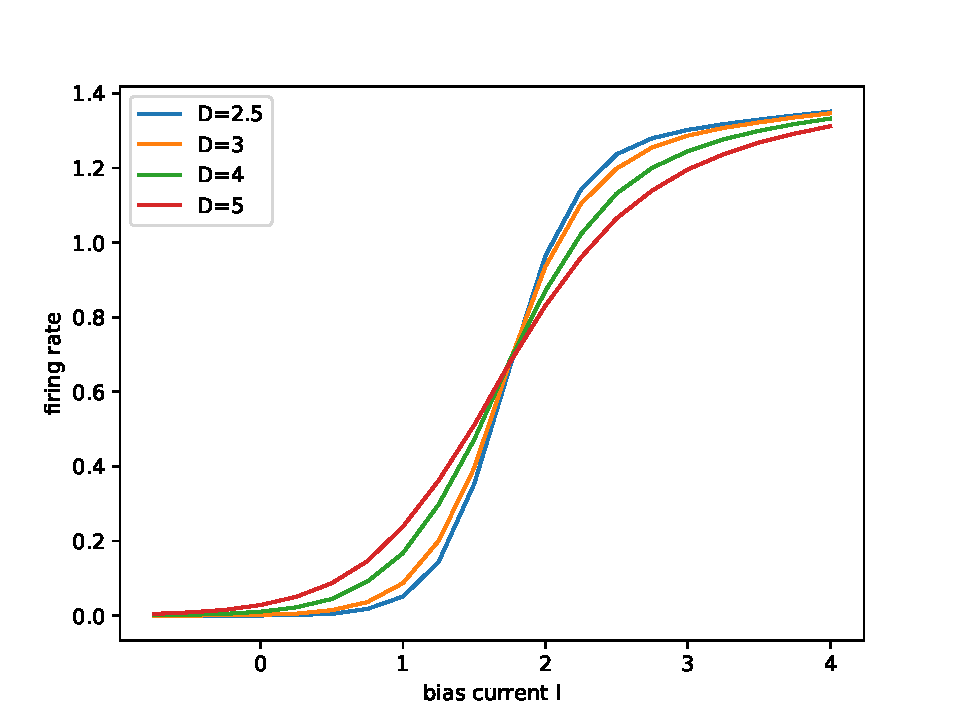
\includegraphics[scale=0.6]{gneurp29m.pdf}
\end{figure}
\end{frame}
\begin{frame}{Simulation: Diffusionskoeffizient}
\begin{figure}	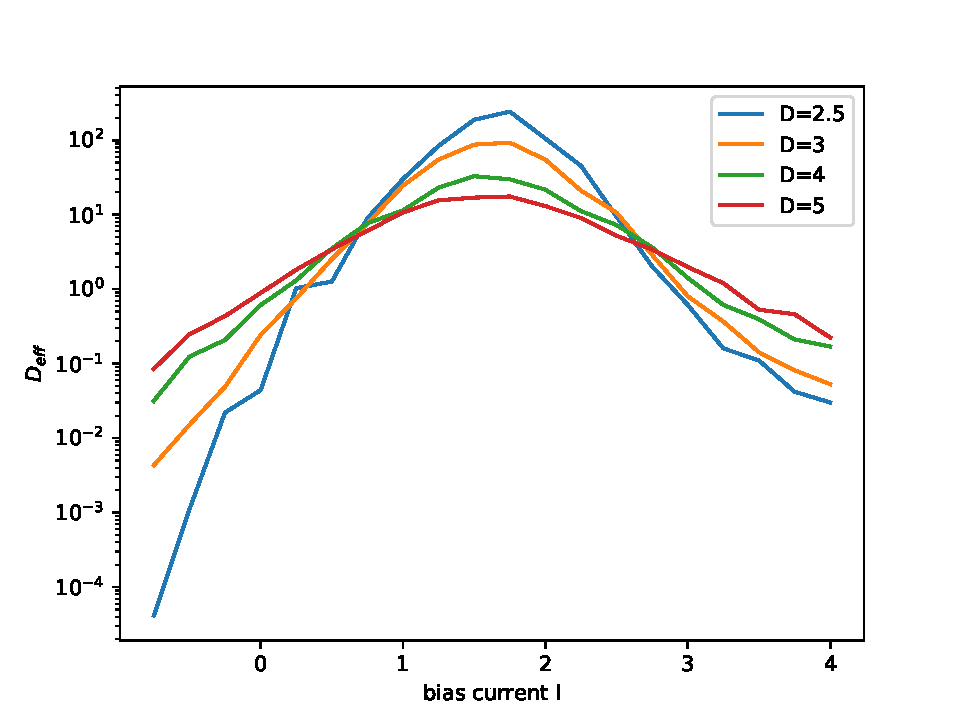
\includegraphics[scale=0.6]{dneurp29m.pdf}
\end{figure}
\end{frame}
\begin{frame}{Simulation: Fano-Faktor}
\begin{figure}	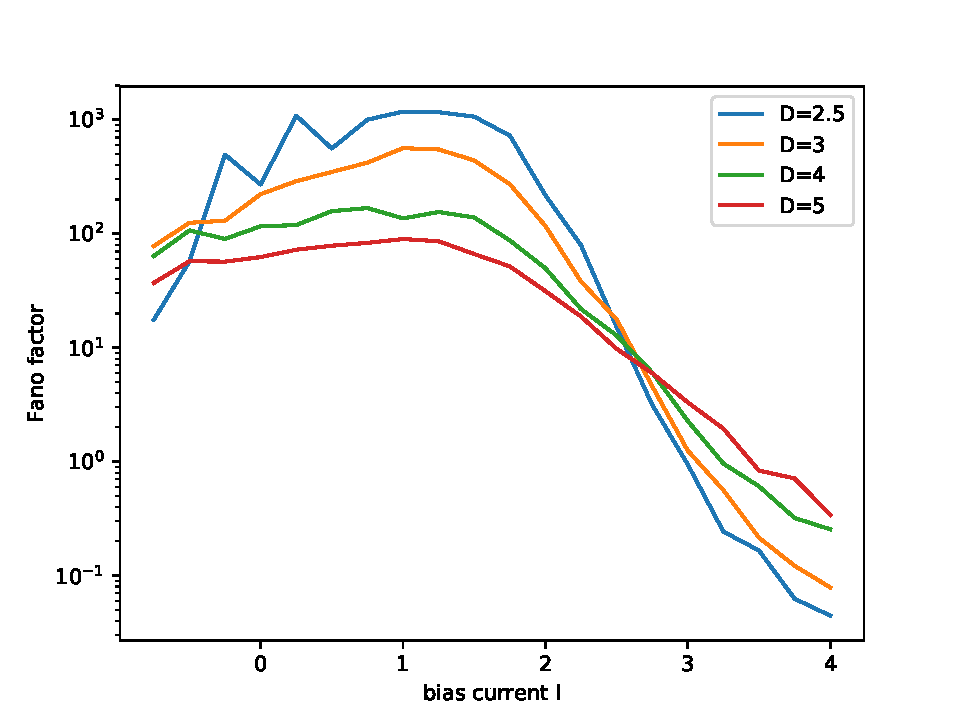
\includegraphics[scale=0.6]{fneurp29mc.pdf}
\end{figure}
\end{frame}
\subsection{Auswertung}
\begin{frame}{Anzahl der "Uberg"ange}
\begin{figure}	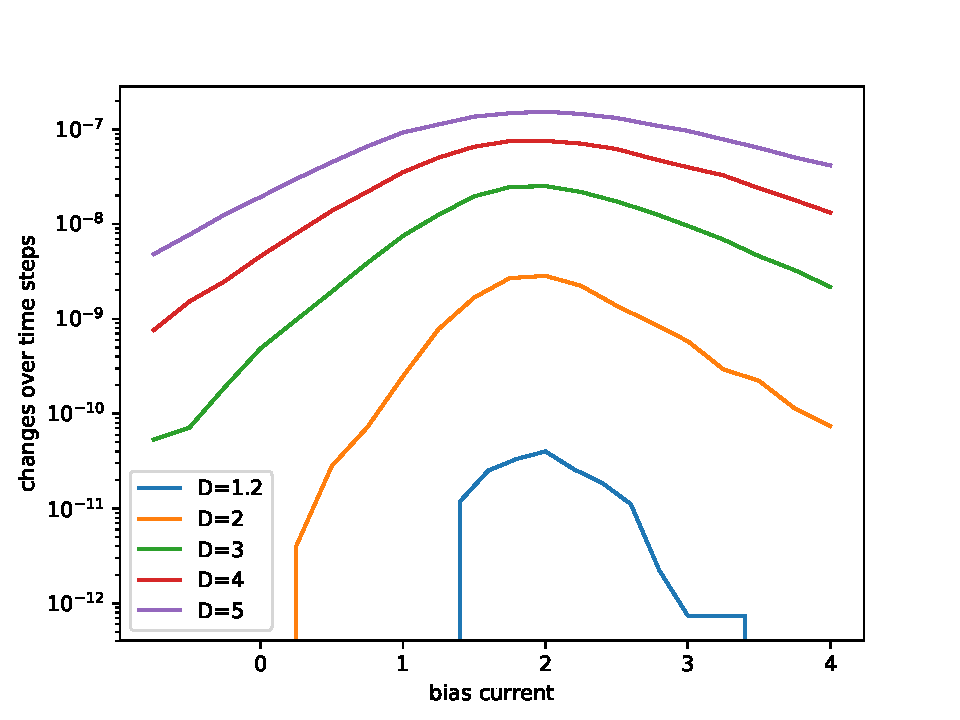
\includegraphics[scale=0.6]{changespertime1m.pdf}
\end{figure}
\end{frame}
\begin{frame}{Arrhenius-Fit}
\begin{figure}	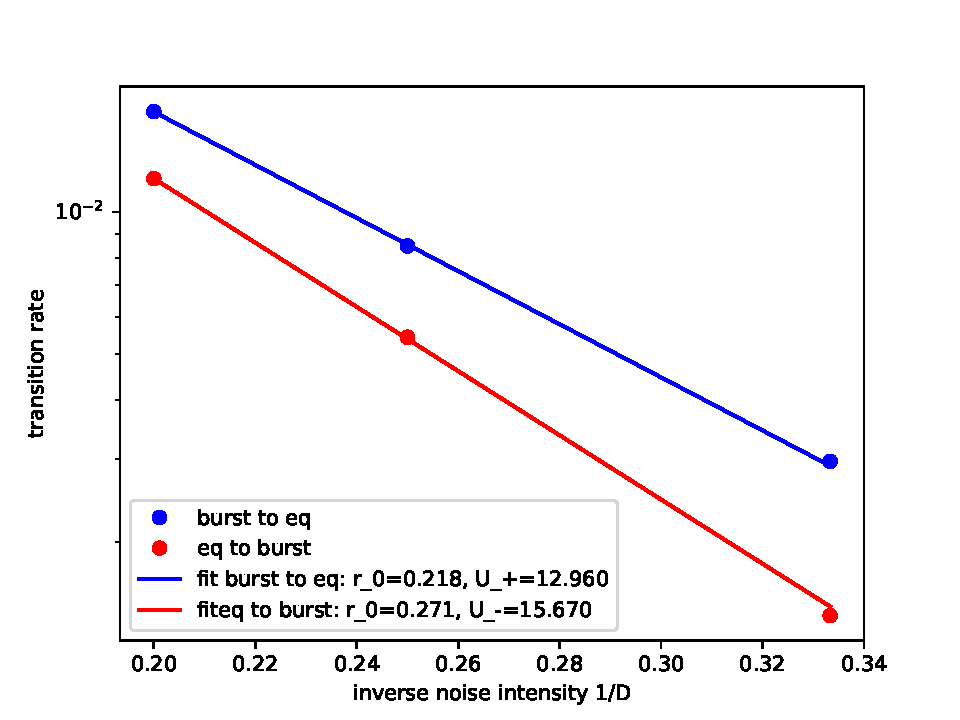
\includegraphics[scale=0.6]{arrheniustot29mfit9.pdf}
\end{figure}
\end{frame}
\begin{frame}{Barrieren f"ur verschiedene Str"ome}
\begin{figure}	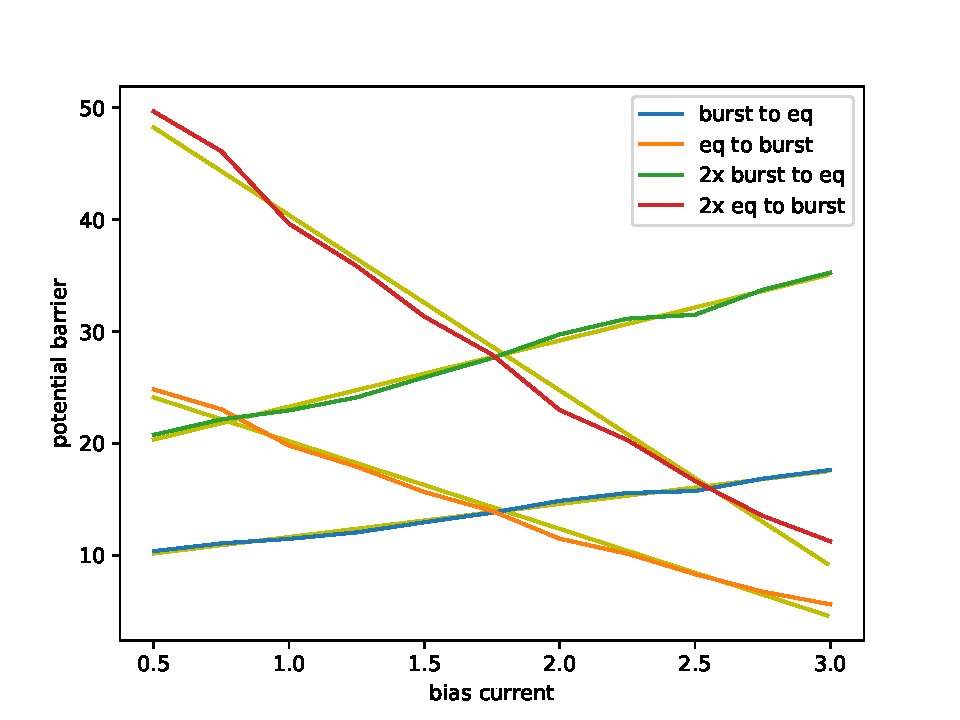
\includegraphics[scale=0.6]{barriercomp29m.pdf}
\end{figure}
\end{frame}
\begin{frame}{Wiederholung: Zwei-Zustands-System}
\begin{itemize}
	\item "Ubergangsraten:
\begin{align*}
r_{\pm}=r_{0,\pm}\text{e}^{-\frac{\Delta U_{\pm}}{Q}}
\end{align*}
\item aus Fits:
\begin{align*}
r_{0,\pm}&=const\\
\Delta U_\pm&=a_\pm\cdot I+b_\pm
\end{align*}

	\item $D_{\text{eff}}$ und $F$ aus Raten und $\Delta v=v_+-v_-$:
\end{itemize}
\begin{align*}
D_{\text{eff}}&=\frac{v_+^2 r_+r_-}{(r_++r_-)^3}\\
F&=\frac{2v_0r_+}{(r_++r_-)^2}
\end{align*}
\end{frame}
\begin{frame}{Vergleich mit Zwei-Zustands-Modell: $D_{eff}$}
\begin{figure}	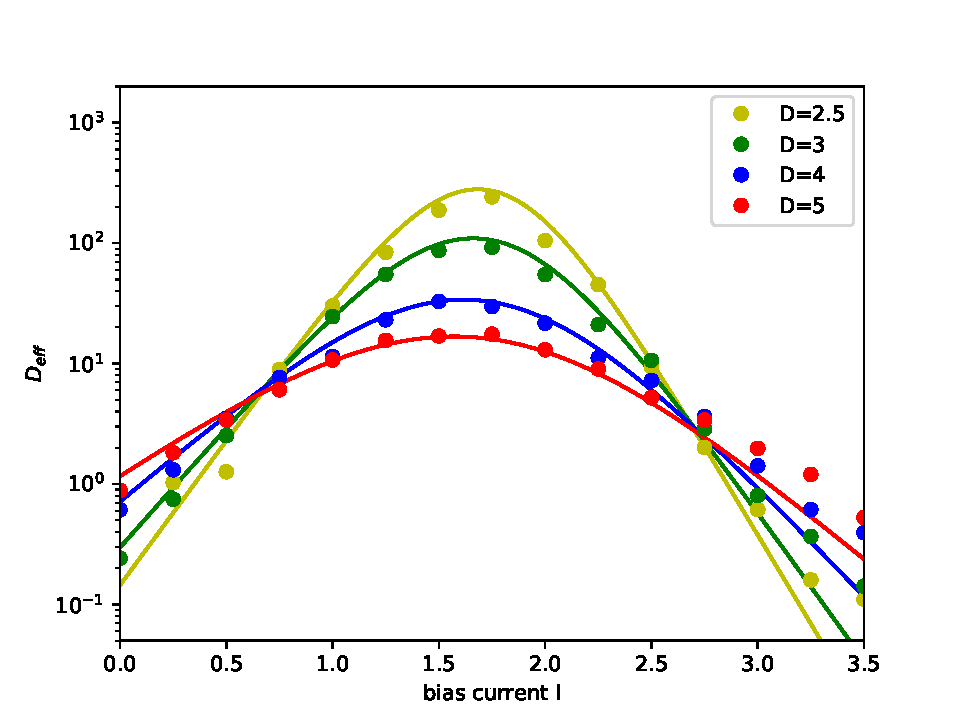
\includegraphics[scale=0.6]{dcompdf29m.pdf}
\end{figure}
\end{frame}
\begin{frame}{Vergleich mit Zwei-Zustands-Modell: $F$}
\begin{figure}	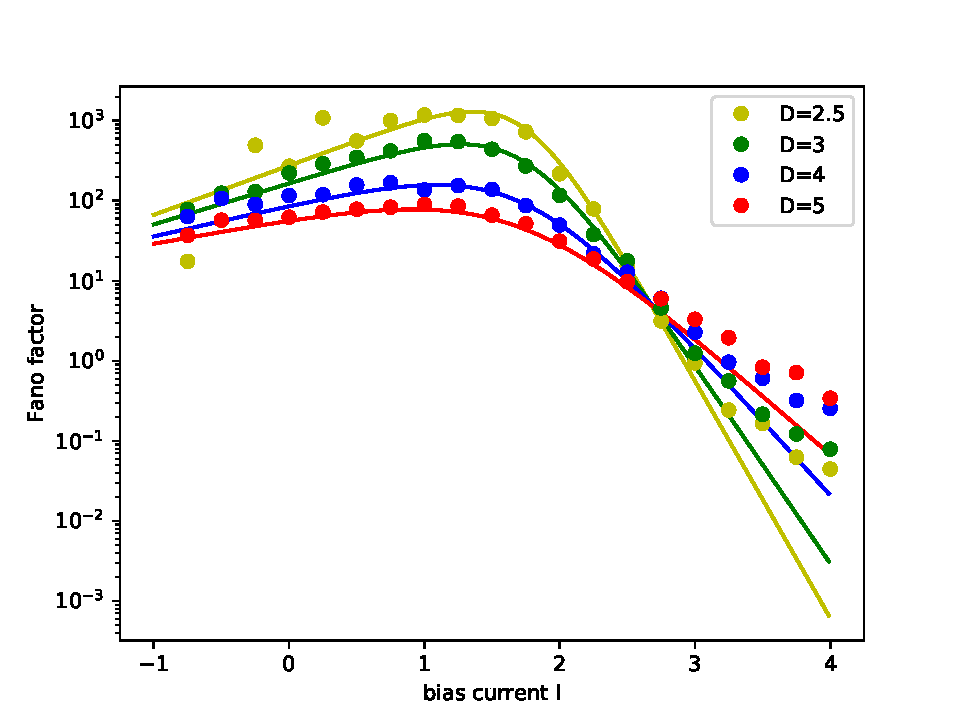
\includegraphics[scale=0.6]{fcompdf29m.pdf}
\end{figure}
\end{frame}
\begin{frame}{Spektrum mit schwachem periodischen Signal}
\begin{figure}	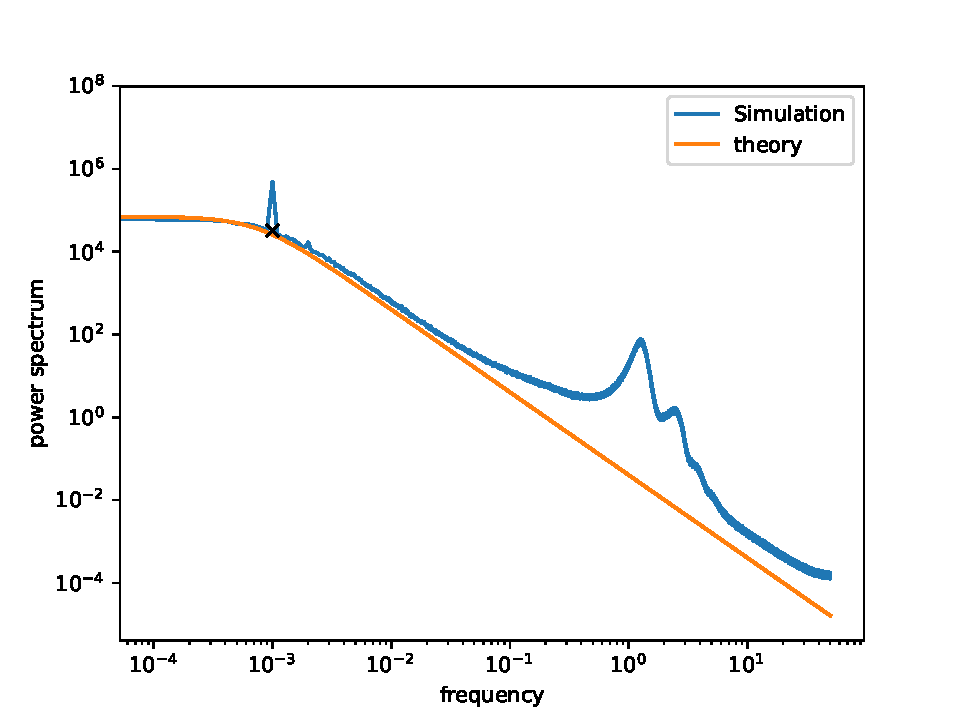
\includegraphics[scale=0.62]{inapik8jlongsnr3010wf.pdf}
\end{figure}

\end{frame}
\begin{frame}{Spektrum mit schwachem periodischen Signal}
\begin{figure}	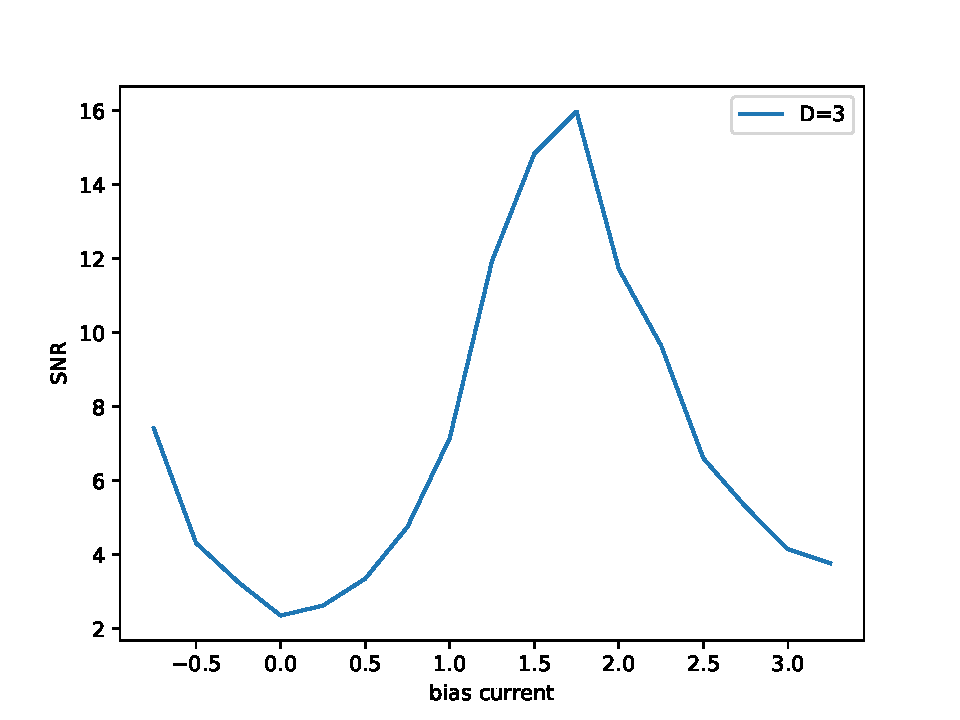
\includegraphics[scale=0.62]{snr3.pdf}
\end{figure}
\end{frame}
\begin{frame}{Vergleich mit $D_{eff}$, Feuerrate}
\begin{figure}	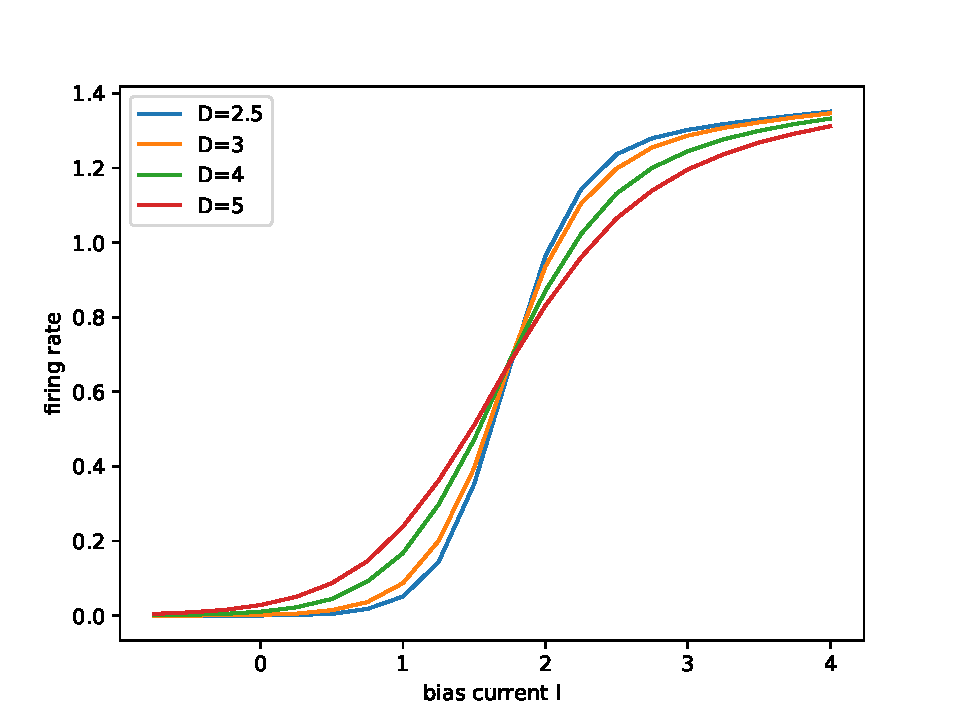
\includegraphics[width=0.7\textwidth,height=0.2\textwidth]{gneurp29m.pdf}
\end{figure}
\vspace{-1cm}
\begin{figure}	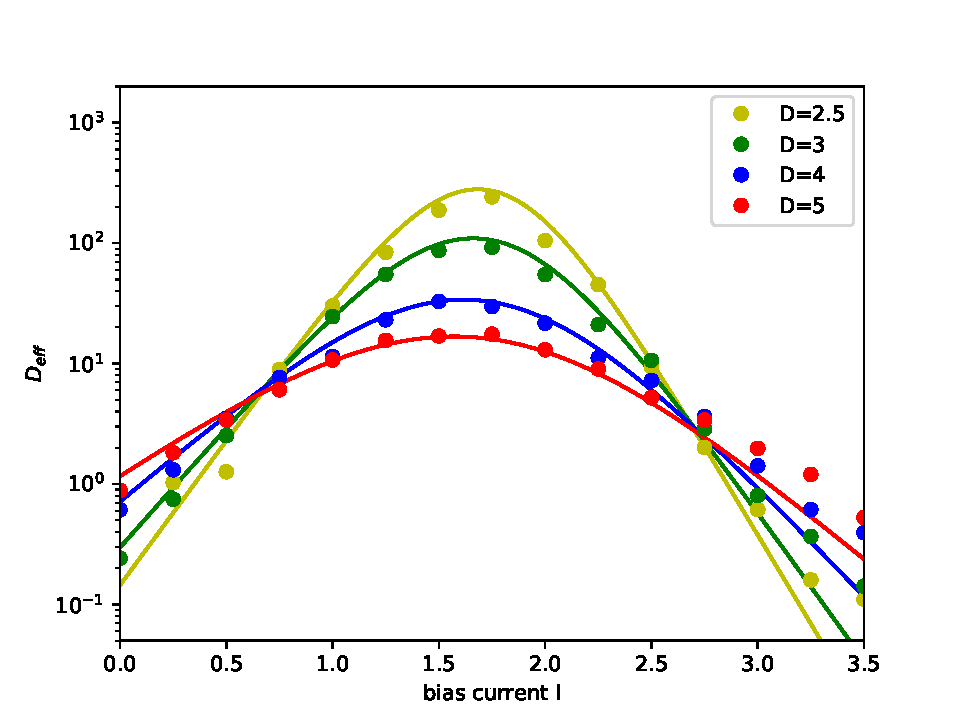
\includegraphics[width=0.7\textwidth,height=0.4\textwidth]{dcompdf29m.pdf}
\end{figure}

\end{frame}
\section{Zusammenfassung}
\begin{frame}{Zusammenfassung und Ausblick}
\begin{itemize}
	\item analog zu Brownschen Teilchen wurde im Nervenmodell ein Bereich gefunden, in dem Giant Diffusion auftritt
	\item kritische Punkte, an denen $D_{eff}$ von Rauschen unabh"angig
	\item Zwei-Zustands-Theorie liefert gute Beschreibung
	\\
	\item als n"achstes: Untersuchung der Abh"angigkeit des SNR von Rauschintensit"at
\end{itemize}
\end{frame}
\end{document}

